%Dokumentenklasse "scrbook" - Erweitert um den Verweis auf die Verzeichnisse und Texteigenschaften
\documentclass[chapterprefix=false, 12pt, a4paper, oneside, parskip=half, listof=totoc, bibliography=totoc, numbers=noendperiod]{scrbook}

% Ränder (Standard bottom ca. 52mm anbzüglich von ca. 4mm für die nach oben rechts gewanderte Seitenzahl)
%Anpassung der Seitenränder
\usepackage[bottom=48mm,left=25mm,right=25mm]{geometry}

% Ränder bei Bedarf zeigen
%\usepackage{showframe}

%Tweaks für scrbook
%\usepackage{scrhack}

%Ermöglicht Verknüpfungen innerhalb des Dokumentes (e.g. for PDF), Links werden durch "hidelink" nicht explizit hervorgehoben
\usepackage[hidelinks,german]{hyperref}
\def\UrlBreaks{\do\/\do-}

%Erlaubt unteranderem Umbrücke captions
\usepackage{caption}
\usepackage{blindtext}

%Stichwortverzeichnis
\usepackage{imakeidx}
\usepackage{subcaption}

\usepackage{lipsum}

%Kompakte Listen
\usepackage{paralist}

%Zitate besser formatieren und darstellen
\usepackage{epigraph}

%Glossar, Stichworverzeichnis
\usepackage[toc, acronym]{glossaries} % Akronyme werden als eigene Liste aufgeführt

%Anpassung von Kopf- und Fußzeile
%beinflusst die erste Seite des Kapitels
\usepackage[automark,headsepline]{scrlayer-scrpage}
\automark{chapter}
\ihead{\leftmark}
\chead{}
\ohead{\thepage}
\ifoot*{}
\cfoot[\thepage]{}
\cfoot*{}
\ofoot*{}
\pagestyle{scrheadings}

\usepackage{multicol}

\renewcaptionname{ngerman}{\contentsname}{Inhalt}
\renewcaptionname{ngerman}{\listfigurename}{Abbildungen}
\renewcaptionname{ngerman}{\listtablename}{Tabellen}
\renewcaptionname{ngerman}{\figurename}{Abb.}
\renewcaptionname{ngerman}{\tablename}{Tab.}

%Auskommentieren für die Verkleinerung des vertikalen Abstandes eines neuen Kapitels
%\renewcommand*{\chapterheadstartvskip}{\vspace*{.25\baselineskip}}

%Zeilenabstand 1,5
\usepackage[onehalfspacing]{setspace}

%Verbesserte Darstellung der Buchstaben zueinander
\usepackage[stretch=10]{microtype}

%Deutsche Bezeichnungen für angezeigte Namen (z.B. Innhaltsverzeichnis etc.)
\usepackage[ngerman]{babel}

%Unterstützung von Umlauten und anderen Sonderzeichen (UTF-8)
\usepackage{lmodern}
\usepackage[utf8]{inputenc}
\usepackage[T1]{fontenc}

%Einfachere Zitate
\usepackage{epigraph}

%Verwendung von Akronymen
\usepackage[printonlyused]{acronym}

%Unterstützung der H positionierung (keine automatische Verschiebung eingefügter Elemente)
\usepackage{float} 

%Erlaubt Umbrüche innerhalb von Tabellen
\usepackage{tabularx}

%Erlaubt Seitenumbrüche mit Tabellen
\usepackage{longtable}

%Erlaubt die Darstellung von Sourcecode mit Highlighting
\usepackage{listings}

%Definierung eigener Farben bei nutzung eines selbst vergebene Namens
\usepackage[table,xcdraw]{xcolor}
\usepackage{color}
\usepackage{tikzpagenodes}

\usepackage[all]{tcolorbox}

%Vektorgrafiken
\usepackage{tikz}

%Grafiken (wie jpg, png, etc.)
\usepackage{graphicx}
\newcommand*{\quelle}[1]{\par\raggedleft\footnotesize Quelle:~#1}

%Grafiken von Text umlaufen lassen
\usepackage{wrapfig}

%Einbindung und Verwaltung von Literaturverzeichnissen
\usepackage{csquotes} %wird von biber benötigt
\usepackage[style=numeric-comp, backend=biber, bibencoding=ascii]{biblatex}
\ExecuteBibliographyOptions{sorting=nty} % Standard
\ExecuteBibliographyOptions{%
  isbn=false, url=false, doi=false, eprint=false,%
}%
\ExecuteBibliographyOptions{%
  firstinits=true,
}%

%\addbibresource{references/references.bib}
\addbibresource{references/literaturN.bib}

%-------------------------------Zusätzliche Anpassungen und Modifikationen--------------------------------------------%

%Anpassung der Überschriften
\addtokomafont{disposition}{\rmfamily}

%Pluszeichen in der Referenc beim zitieren ausblenden
\renewcommand*{\labelalphaothers}{}

%Anpassungen für das Abkürzungsverzeichnis
%\newglossarystyle{dottedlocations}{%
%	\glossarystyle{list}%
%	\renewcommand*{\glossaryentryfield}[5]{%
%		\item[\glsentryitem{##1}\glstarget{##1}{##2}] \emph{##3}%
%		\unskip\leaders\hbox to 2.9mm{\hss.}\hfill##5}%
%	\renewcommand*{\glsgroupskip}{}%
%}

\setcounter{secnumdepth}{4}
\setcounter{tocdepth}{4}

%include the usecases package
\usepackage{usecases}

\usepackage{color}

\usepackage{tcolorbox}
%\tcbuselibrary{listings,skins}        %%% skins needed for shadow

\definecolor{lbcolor}{rgb}{0.1,0.1,0.1}
\definecolor{bg}{rgb}{0.85,0.85,0.85}

\usepackage{etoolbox}
%
%\pretocmd{\chapter}{\addtocontents{mybox}{\addvspace{5pt}}}{}{}
%\makeatletter
%\renewcommand*{\@chapterlistsgap}{0\p@}
%\renewcommand*\l@tcolorbox{\@dottedtocline{1}{1.5em}{3em}}
%\makeatother

%\makeatletter
%\renewcommand*{\@chapterlistsgap}{0\p@}
%\makeatother

\makeatletter
\patchcmd{\@chapter}
  {\chaptermark{#1}}% search
  {\chaptermark{#1}\addtocontents{mybox}{\protect\addvspace{10\p@}}}% replace
  {}{}
  \renewcommand*\l@tcolorbox{\@dottedtocline{1}{1.5em}{2.3em}}
\makeatother

\newminted[myjson]{js}{tabsize=2,fontsize=\footnotesize}
\newminted[myxml]{xml}{tabsize=2,fontsize=\footnotesize}
\newminted[myshell]{shell-session}{tabsize=2,fontsize=\footnotesize}
\newminted[mycode]{text}{tabsize=2,fontsize=\footnotesize}
\newminted[myJava]{java}{tabsize=2,fontsize=\footnotesize, linenos, numbersep=3mm}
\newminted[myJS]{javascript}{tabsize=2,fontsize=\footnotesize}

% Box for Shell
\newtcolorbox[auto counter,number within=chapter,
  list inside=mybox]{mintedboxShell}[2][]{%
  title={Listing \thetcbcounter: #2},
  list entry={\protect\numberline{\thetcbcounter}#2},
  enhanced,
  left=6mm,
  overlay={\begin{tcbclipinterior}\fill[black!5!white] (frame.south west)
            rectangle ([xshift=6mm]frame.north west);\end{tcbclipinterior}},
  colframe=black!50!black,
  colback=black!5!white,
  drop fuzzy shadow,#1}
  
\newenvironment{listingsboxShell}[3][]
 {%
   \def\listingsboxenvironment{#2}%save the environments
   \VerbatimEnvironment%
   \begin{mintedboxShell}[#1]{#3}%
     \begin{\listingsboxenvironment}}%
 {%
  \end{\listingsboxenvironment}%
  \end{mintedboxShell}%
}

% Box for Java
\newtcolorbox[auto counter,number within=chapter,
  list inside=mybox]{mintedboxJava}[2][]{%
  title={Listing \thetcbcounter: #2},
  list entry={\protect\numberline{\thetcbcounter}#2},
  enhanced,
  left=6mm,
  overlay={\begin{tcbclipinterior}\fill[red!5!white] (frame.south west)
            rectangle ([xshift=6mm]frame.north west);\end{tcbclipinterior}},
  colframe=red!75!black,
  colback=red!5!white,
  drop fuzzy shadow,#1}

\newenvironment{listingsboxJava}[3][]
 {%
   \def\listingsboxenvironment{#2}%save the environments
   \VerbatimEnvironment%
   \begin{mintedboxJava}[#1]{#3}%
     \begin{\listingsboxenvironment}}%
 {%
  \end{\listingsboxenvironment}%
  \end{mintedboxJava}%
}

% Box for JavaScript
\newtcolorbox[auto counter,number within=chapter,
  list inside=mybox]{mintedboxJavaScript}[2][]{%
  title={Listing \thetcbcounter: #2},
  list entry={\protect\numberline{\thetcbcounter}#2},
  enhanced,
  left=6mm,
  overlay={\begin{tcbclipinterior}\fill[green!5!white] (frame.south west)
            rectangle ([xshift=6mm]frame.north west);\end{tcbclipinterior}},
  colframe=green!75!black,
  colback=green!5!white,
  drop fuzzy shadow,#1}

\newenvironment{listingsboxJavaScript}[3][]
 {%
   \def\listingsboxenvironment{#2}%save the environments
   \VerbatimEnvironment%
   \begin{mintedboxJavaScript}[#1]{#3}%
     \begin{\listingsboxenvironment}}%
 {%
  \end{\listingsboxenvironment}%
  \end{mintedboxJavaScript}%
}

\makeatletter

\newcommand*{\gradeType}[1]{\gdef\@gradeType{#1}}
\newcommand*{\firstExaminer}[1]{\gdef\@firstExaminer{#1}}
\newcommand*{\secondExaminer}[1]{\gdef\@secondExaminer{#1}}
\newcommand*{\matrikelnr}[1]{\gdef\@matrikelnr{#1}}
\newcommand*{\submitDate}[1]{\gdef\@submitDate{#1}}
\newcommand*{\handlingPeriod}[1]{\gdef\@handlingPeriod{#1}}
\newcommand*{\address}[1]{\gdef\@address{#1}}
\newcommand*{\thema}[1]{\gdef\@thema{#1}}
\newcommand*{\themaPartTwo}[1]{\gdef\@themaPartTwo{#1}}
\newcommand{\themaT}{Architektur für skalierbare Webanwendungen}
\newcommand{\Cap}{\textbf{C}onsistency (Konsistenz)}
\newcommand{\cAp}{\textbf{A}vailability (Hochverfügbarkeit)}
\newcommand{\caP}{\textbf{P}artition Tolerance (Partitionstoleranz)}
\newcommand{\CA}{\textbf{C}onsistency (Konsistenz) und \textbf{A}vailability (Hochverfügbarkeit)}
\newcommand{\CP}{\textbf{C}onsistency (Konsistenz) und \textbf{P}artition Tolerance (Partitionstoleranz)}
\newcommand{\AP}{\textbf{A}vailability (Hochverfügbarkeit) und \textbf{P}artition Tolerance (Partitionstoleranz)}
\newcommand{\acid}{\textbf{ACID-}Prinzip}
\newcommand{\Acid}{\textbf{A}tomicity (Atomarität)}
\newcommand{\aCid}{\textbf{C}onsistency (Konsistenz)}
\newcommand{\acId}{\textbf{I}solation (Isolation)}
\newcommand{\aciD}{\textbf{D}urability (Dauerhaftigkeit)}
\newcommand{\BAse}{\textbf{B}asically \textbf{A}vailable}
\newcommand{\baSe}{\textbf{S}oft State}
\newcommand{\basE}{\textbf{E}ventually Consistent}

\renewcommand*{\maketitle}{
	\begin{titlepage}
		\newgeometry{left=2.5cm,right=2.5cm,top=4.0cm,bottom=2.5cm}
		\begin{center}
		
\includegraphics[width=0.8\textwidth]{resources/HMLogoFK07.png}
			\vfill
		%\vskip 0.5cm
			{\Large \@thema}
			\vskip 0.3cm
			{\Large \@themaPartTwo}
			\vskip 0.5cm
			{\large \bfseries Bachelor-Thesis\par}
			\vskip 0.5cm
			{\large zur Erlangung des akademischen Grades}
			\vskip 0.5cm
			{\large \textit{\bfseries \@gradeType}}
			\vskip 0.5cm
			{\large im Studiengang Wirtschaftsinformatik}
			\vskip 0.0cm
			{\large an der}
			\vskip 0.0cm
			{\large Hochschule für angewandte Wissenschaften München\\Fakultät für Informatik und Mathematik}
			\vfill
			\begin{center}
				\begin{tabular}[t]{lr}
					\textsc{Betreuer:} &\@firstExaminer\\
					\textsc{Vorgelegt von:} &\@author\\
					&\@address\\
					\textsc{Matrikelnummer:} & \@matrikelnr\\
					\textsc{Bearbeitungszeit:} & \@handlingPeriod\\
					\textsc{Eingereicht am:} & \@submitDate\\
				\end{tabular}
			\end{center}
		\end{center}
		\restoregeometry
	\end{titlepage}
}
\makeatother
\gradeType{Bachelor of Science (B.Sc.)}

%%Used by all titles
\thema{\textsc{Architektur}}
\themaPartTwo{\textsc{für skalierbare Webanwendungen}}
\author{Vladislav Faerman}
\address{Waldstr. 7, 82024 Taufkirchen}
\matrikelnr{02929612}
%\handlingPeriod{10.01.2017 bis 25.02.2017}
\handlingPeriod{3 Monate}
\submitDate{28.02.2017}
\firstExaminer{Prof. Dr. Oliver Braun}
%%End Titles

\makeindex[title=Stichwortverzeichnis, options=-s indexstyle.ist, intoc]
\indexsetup{level=\chapter*,toclevel=chapter}

\begin{document}
\input{chapter/ToDo} \clearpage

\pagenumbering{alph}
%\maketitle

\pagenumbering{Roman}

%%\addchap{Eigenständigkeitserklärung}
%\addchap{Eidesstattliche Erklärung}
\chapter*{Eidesstattliche Erklärung}

 
Hiermit versichere ich, dass ich die vorliegende Arbeit '\themaT' selbstständig und keine anderen als die angegebenen Quellen und Hilfsmittel benutzt habe. Alle Stellen, die wörtlich oder sinngemäß aus Veröffentlichungen entnommen sind, habe ich als solche kenntlich gemacht. Diese Arbeit ist bislang keiner anderen Prüfungsbehörde vorgelegt worden und auch nicht veröffentlicht worden.
\\\\München, 24. April 2017

\vskip 1.5cm

\underline{~~~~~~~~~~~~~~~~~~~~~~~~}\\
Vladislav Faerman\\
%\chapter*{Danksagung}

Lieber Bruder, liebe Eltern, lieber Familie, lieber Prof. Dr. Braun,

mit dieser Bachelorarbeit neigt sich meine Studienzeit an der Hochschule München dem Ende zu. Während meiner Studienzeit habe ich blabla.......

Mein größter Dank gilt meinen Eltern, meinem älteren Bruder und meiner Familie, die mich stets unterstützt haben.

Die Zusammenarbeit mit meinem älteren Bruder Evgeniy Faerman war von großer Hilfsbereitschaft geprägt und möchte ich nicht unerwähnt lassen. Ich bedanke mich auch hanz herzlich bei dir. Du hast mir nicht nur der Korrektur dieser Arbeit Herausragendes geleistet. Ohne dich wäre diese Arbeit nicht in dieser Form zustande gekommen.

Bei meinem Professor Dr. Oliver Braun möchte ich mich auch recht herzlich bedanken, der es mir ermöglicht hat, meine Abschlussarbeit bei ihm zu Ende zu bringen. Ich bedanke mich für die Betreuung und Begutachtung der Bachelorarbeit.

\vskip 1.5cm

\underline{~~~~~~~~~~~~~~~~~~~~~~~~}\\
Vladislav Faerman\\

  \clearpage
%\chapter*{Vorwort}
\blindtext \clearpage
\tableofcontents \newpage
\pagenumbering{arabic}
%%\chapter{Einleitung}
\chapter{\colorbox{green}{Einleitung}}

Internetnutzer erwarten heutzutage von den Webanwendungen, dass diese kurze Ladezeiten, flüssige selbsterklärende Bedienung und ständige Verfügbarkeit aufweisen. Viele Webanwendungen sind nicht in der Lage, mit rasant steigender Anzahl von Anfragen und großen Datenmengen effizient umzugehen.

Dies ist für erfolgreiche Projekte, die rapide populär werden und ein exponentielles Anwenderwachstum erleben, ein ernsthaftes Problem. Um von dem Projekterfolg profitieren zu können und diesen auszubauen, ist es überlebenswichtig, den Wachstumsanforderungen gerecht zu werden. Die Hardware stellt gegenwärtig kein großes Problem mehr dar: Die Cloud-Services wie z. B. \textit{Amazon} oder \textit{Microsoft Azure} ermöglichen den Zugang zu den fast unbegrenzten Hardwareressourcen. Die Herausforderung für Entwickler besteht darin, die Webanwendung so zu bauen, dass diese von dem Hardwareangebot Gebrauch machen kann. Die Wartungs- und Erweiterungsfähigkeit sind zwei weiteren wichtigen Punkte, die für den Erfolg unabdingbar sind. Um die Internetnutzer beizubehalten, sollen die neuen Features schnell implementiert und ausgerollt werden können, auch wenn das Projekt größer wird.

%\section{Motivation und Ziel der Arbeit}
\section{\colorbox{green}{Motivation und Ziel der Arbeit}}

Das Ziel dieser Arbeit ist, eine solche Architektur für Webanwendungen vorzustellen, die die Entwicklung von skalierbaren, wartungs- und erweiterungsfähigen Webanwendungen ermöglicht. Es wird des Weiteren ein Software-  und Frameworkstack vorgeschlagen, der diese Architektur abdeckt. Die vorgeschlagenen Software/Frameworks sind unter freien Lizenzen verfügbar.

Um die Realisierbarkeit und das Zusammenspiel aller Komponenten zu untersuchen, wird ein Prototyp implementiert und eigene Erfahrungen aus dem Entwicklungsprozess berichtet. Für den Prototyp wird der webbasierte Foto-Verwaltungs-Service gewählt. Diese Anwendung zeichnet sich dadurch aus, dass jeder Internetnutzer eigene Daten unabhängig von den anderen Nutzern verwalten kann, was bei vielen Webanwendungen der Fall ist. Anderenfalls sollen nicht nur triviale Textdaten verwaltet werden, sondern auch mehrere Dateien.
%\section{Aufbau der Arbeit}
%Erst Grundlagen/Konzepte, die relevant sind, um eine skalierbare und wartbare Webapplikation implementieren zu können.

%\section{Codeimplementierung}

%Der sämtliche Source Code liegt in dem folgenden GitHub Repository:

%\url{https://github.com/vlxxxfa/vlxxxfa.github.io} \clearpage
%\chapter{Software-Architektur}
Drei-Schichten-Modell als Software-Architektur blabla
\colorbox{red}{BILD nur zum Testennnnnnn}
\begin{figure}
\centering
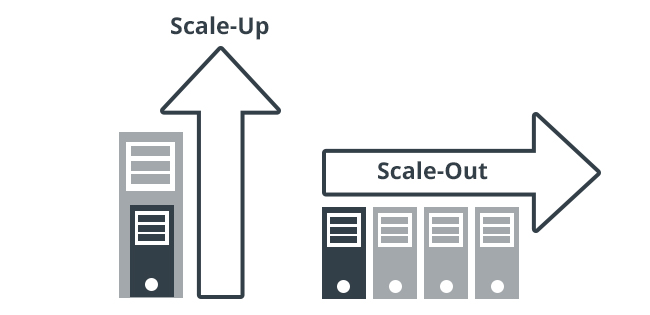
\includegraphics[width=0.7\textwidth]{resources/scales}
\caption[TEST]{TEST\protect\footnotemark}
\label{img:scales}
\end{figure}
\footnotetext{TEST: \url{https://magazin.kapilendo.de/den-supergau-verhindern-so-bereiten-sie-ihre-website-auf-einen-besucheransturm-vor/}, zugegriffen am 15. Januar 2017}

\section{Allgemein} \clearpage
\chapter{NoSQL-Systemen}
%\begin{tikzpicture}[remember picture,overlay]
%\node[anchor=east,inner sep=0pt] at (current page text area.east|-0,6cm) %{
\includegraphics[height=4cm]{resources/mongoDBlogo}};
%\end{tikzpicture}
\section{Definition}
Im Vergleich zu den relationalen Datenbanken, die sich als eine strukturierte Sammlung von Tabellen (den Relationen) vorstellen, in welchen Datensätze abgespeichert sind, eignen sich NoSQL Datenbanken zur unstrukturierter Daten, die einen nicht-relationalen Ansatz verfolgen. Typische Beispiele für unstrukturierte Daten sind: Benutzer- und Sitzungsdaten, Chat-, Messaging- und Protokolldaten, Zeitreihendaten wie IoT- und Gerätedaten sowie große Objekte wie Videos und Bilder.\footnote{NSQL-Datenbanken: \url{http://de.basho.com/resources/nosql-databases/}, zugegriffen am 20. Dezember 2016}

Der Begriff NoSQL steht nicht für 'kein SQL', sondern für 'nicht nur SQL' (Not only SQL). Das Ziel von NoSQL ist, relationale Datenbanken sinnvoll zu ergänzen, wo sie Defizite aufzeigen. Entstanden ist dieses Konzept in erster Linie als Antwort zur Unflexibilität, sowie zur relativ schwierigen Skalierbarkeit von klassischen Datenbanksystemen, bei denen die Daten nach einem stark strukturierten Modell gespeichert werden müssen.\footnote{MySQL vs. MongoDB: \url{http://www.computerwoche.de/a/datenbanksysteme-fuer-web-anwendungen-im-vergleich,2496589}, zugegriffen am 22. Dezember 2016} Dokumentdatenbanken gruppieren die Daten in einem strukturierten Dokument, typischerweise in einer JSON-Datenstruktur. Auch MongoDB, siehe dazu Kapitel \ref{mongo} verfolgt diesen Ansatz und bietet darauf aufbauend eine reichhaltige Abfragesprache und Indexe auf einzelne Datenfelder. Die Möglichkeiten der Replikation und des Shardings zur stufenlosen und unkomplizierten Skalierung der Daten und Zugriffe macht MongoDB auch für stark frequentierte Websites äußerst interessant.(\cite{Hollosi.2012}, Kapitel 14, Seite 435)
\subsection{Kategorisierung von NoSQL-Systemen}
Der Abschnitt stellt verschiedene NoSQL-Systemen mit ihren Vor- und Nachteilen vor.
\subsubsection{Dokumentenorientierte Datenbanken}

Siehe Artikel \url{http://pi.informatik.uni-siegen.de/Mitarbeiter/mrindt/Lehre/Seminare/NoSQL/einreichungen/NOSQLTEC-2015_paper_9.pdf}

siehe \cite[S. 5-8]{Edlich.2011}
\subsubsection{Key-Value-Datenbanken}
\subsubsection{Spaltenorientierte Datenbanken}
\subsubsection{Objektdatenbanken}
\subsubsection{Graphdatenbanken}

\section{ACID}
bla

\section{Das CAP-Theorem}


Im Jahr 2000 hielt Brewer\footnote{Eric A. Brewer ist ein Informatik-Professor an der University of California, Berkeley und einer der Erfinder der Suchmaschine Inktomi} die Keynote auf dem ACM Symposium on Principles of Distributed Computing (PODC)\footnote{PODC2000: \url{http://www.podc.org/podc2000/}, zugegriffen am 02.01.2017}, einer Konferenz über die Grundlagen der Datenverarbeitung in verteilten Systemen\footnote{In einem verteilten System im Bereich Datenverarbeitung werden gespeicherte Daten mehrfach über mindestens zwei verschiedene Server repliziert und miteinander synchronisiert, um die Verfügbarkeit der Daten zu erhöhen und die Zugriffszeiten der User zu verringern.} (Principles of Distributed Computing).  In seiner Keynote stellte Brewer sein \textbf{CAP}-Theorem vor, ein Ergebnis seiner Forschungen zu verteilten Systemen an der University of California \cite[S. 13]{Kurowski.2012}. Brewer's Theorem wurde im Jahr 2002 von Seth Gilbert und Nancy Lynch formal bewiesen.

Das Akronym \textbf{CAP} steht für die englischsprachigen Begriffe  \Cap, \cAp\ und \caP\ und beschreiben die Anforderungen für die Skalierung an verteilte Systeme, die es zunächst näher zu erläutern gilt.

Was besagt eigentlich dieses \textbf{CAP}-Theorem? Das \textbf{CAP}-Theorem besagt, dass die verteilten Systeme, die mit großen Datenmengen zu tun haben, gleichzeitig die folgenden Anforderungen wie \Cap, \cAp\ und \caP\ nicht erfüllen können.
%\begin{figure}
%\centering
%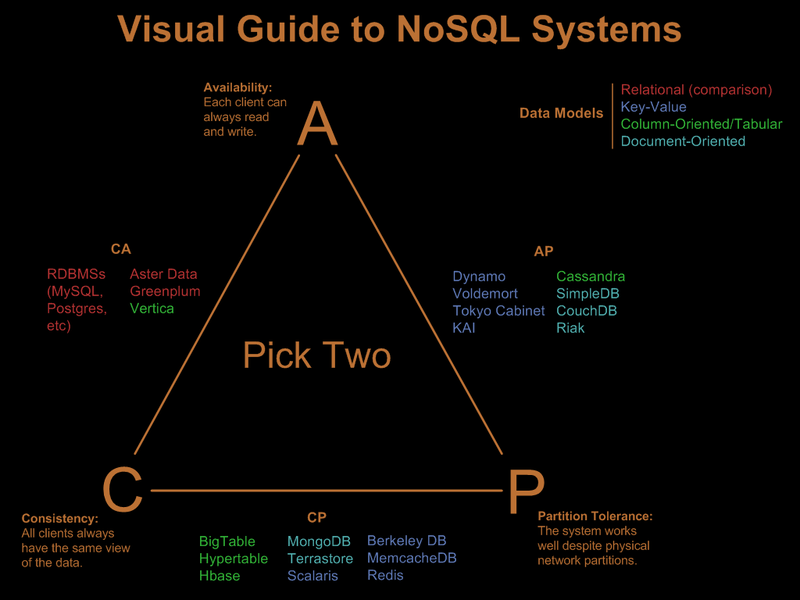
\includegraphics[width=1.0\textwidth]{resources/pickTwoCAP}
%\caption[bla]{CAP Theorem\protect\footnotemark}
%\label{img:cap}
%\end{figure}
%\footnotetext{Visual Guide to NoSQL Systems: \url{http://blog.nahurst.com/visual-guide-to-nosql-systems}, zugegriffen am 27. Dezember 2016}
%\begin{figure}
%\centering
%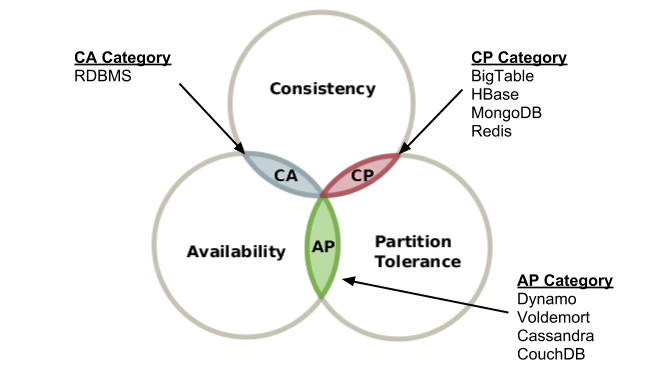
\includegraphics[width=0.8\textwidth]{resources/captheorem2}
%\caption[\capTheorem]{Anforderungen an verteilte Systeme gemäß dem Professor Eric A. Brewer's \capTheorem\protect\footnotemark}
%\label{img:cap}
%\end{figure}
%\footnotetext{CAP Theorem: \url{https://datawarehouseview.wordpress.com/tag/cap-theorem/}, zugegriffen am 23. Dezember 2016}
%

\begin{figure}
\centering
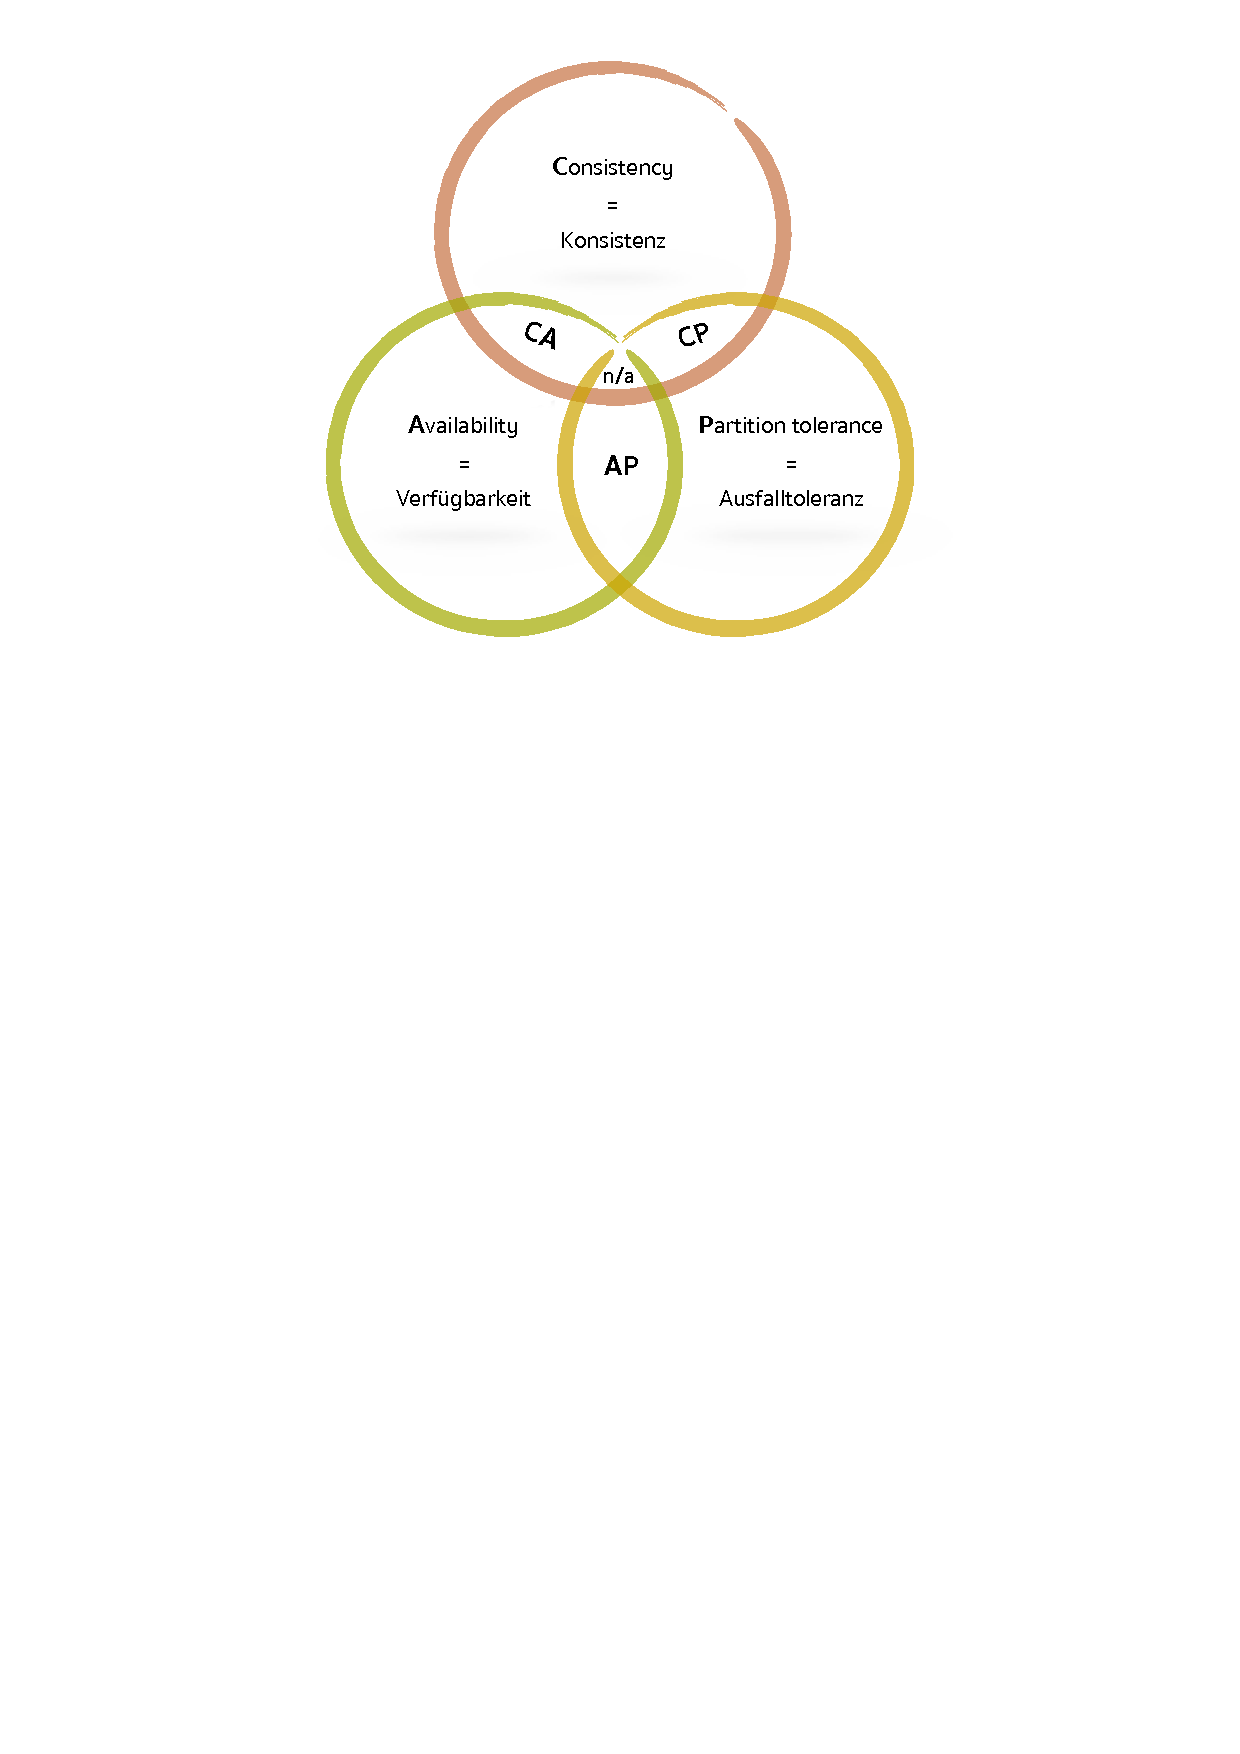
\includegraphics[trim = 0mm 189mm 0mm 9mm, clip, width=1.0\textwidth]{resources/myPictureForCAP}
\caption[\textbf{CAP}-Theorem]{Anforderungen an verteilte Systeme gemäß dem \textbf{CAP}-Theorem}
\label{img:cap}
\end{figure}

%\begin{figure}
%\centering
%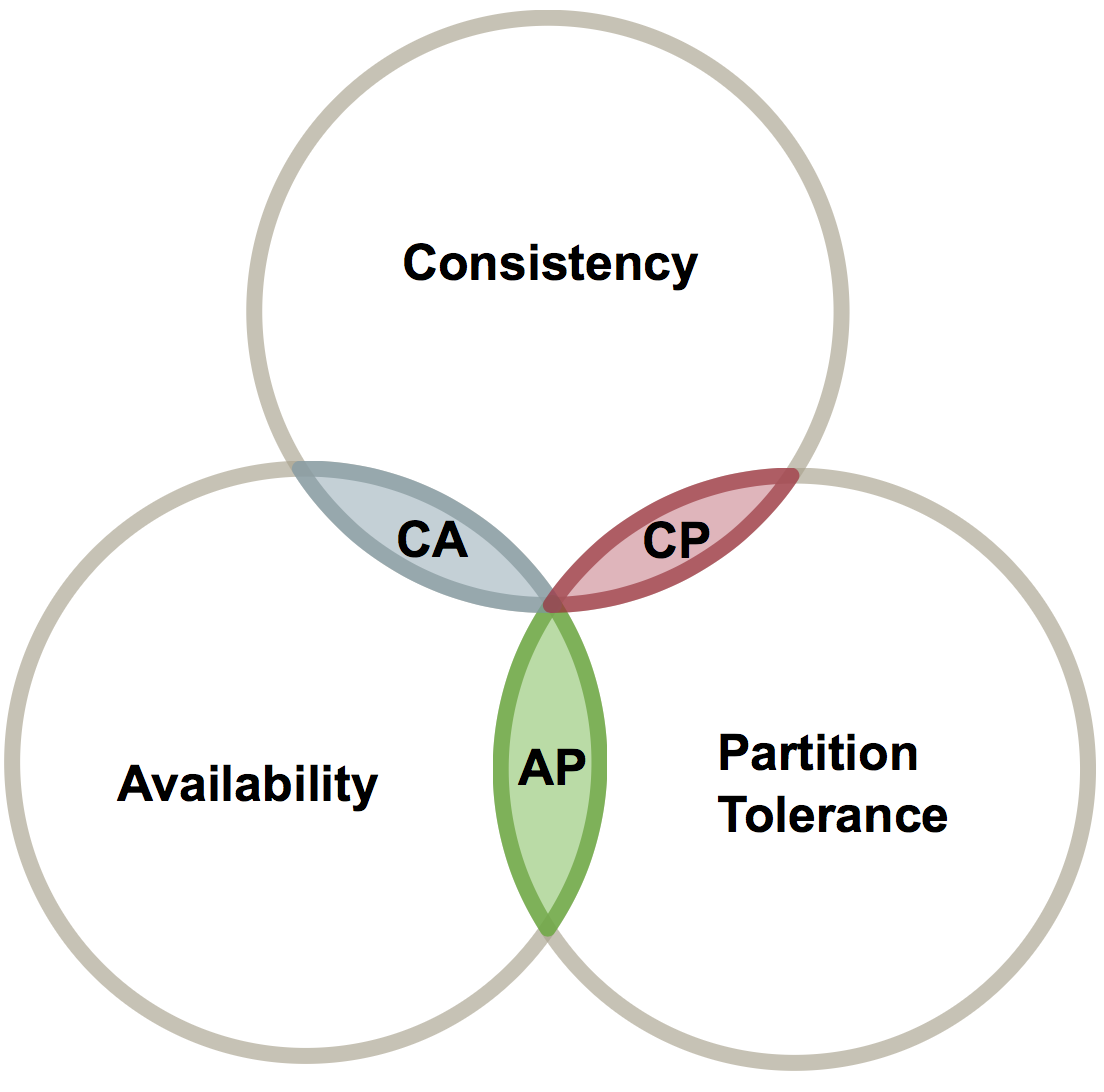
\includegraphics[width=0.5\textwidth]{resources/cap}
%\caption[bla]{CAP Theorem \protect\cite{Brewer.}}
%\label{img:cap}
%\end{figure}

\begin{itemize}
\item \Cap: Die \textit{Konsistenz} der Daten in einem verteilten System bedeutet, dass alle replizierenden Knoten aus einem großen Cluster über die gleiche Datenstruktur verfügen. Falls ein Wert auf einem Knoten durch eine Transaktion per Schreiboperation geändert ist, muss der aktualisierte Wert auf Anfrage mit der Leseoperation von anderen Knoten zurückgeliefert werden können. Die Transaktion selbst ist eine atomare\footnote{Eine atomare Transaktion bedeutet, dass sie entweder ganz oder gar nicht ausgeführt wird. Falls eine atomare Transaktion abgebrochen wird, werden alle im Laufe der Transaktion schon durchgeführte Änderungen rückgängig gemacht.} Einheit in der Datenbank.
%
%\item \Cap: Die \textit{Konsistenz} der gespeicherten Daten beschreibt in einem verteilten Datenbanksystem so einen Datenstand auf den Servern, in dem nach dem Abschluss einer Transaktion alle replizierenden Knoten aus einem großen Cluster über die gleiche Datenstruktur verfügen. Die Transaktion selbst ist eine atomare Einheit in der Datenbank, die entweder als Ganzes erfolgreich verläuft \textbf{(=Commit)} oder durch einen \textbf{Rollback} rückgängig gemacht werden kann.
%
%\textbf{Beispiel für einen konsistenten Zustand der gespeicherten Daten:} In einem verteilten Datenbanksystem mit mehreren replizierenden Knoten sind die Daten nur dann konsistent, wenn auf einem Knoten geänderte Eintrag die alle darauf folgenden Lesezugriffe über andere Cluster den geänderten Wert zurückliefert.
%
%ändert sich nach einer Transaktion auf einem Knoten ein Eintrag in einem Dokument. Um alle folgenden Lesezugriffe, die beispielsweise über andere Knoten aus demselben Cluster ausgeführt w
%
%für einen konsistenten Zustand ändert eine Transaktion in einem Knoten einen Datensatz. Bei erfolgreichem Abschluss der Transaktion muss der geänderte Wert in einem verteilten Datenbanksystem mit mehreren replizierenden Knoten bei der Anfrage von jedem Knoten zurückgeliefert werden können.
%
\item \cAp: Die \textit{Hochverfügbarkeit} ist die weitere Anforderung, die besagt, dass immer alle gesendeten Anfragen durch User ans System beantwortet werden müssen und mit einer akzeptablen Reaktionszeit.
\item \caP: Die \textit{Partitions- oder Ausfalltoleranz} bedeutet, dass der Ausfall eines Knoten bzw. eines Servers aus einem Cluster das verteilte System nicht beeinträchtigt und es fehlerfrei weiter funktioniert. Falls einzelne Knoten in so einem System ausfallen, wird deren Ausfall von den verbleibenden Knoten aus dem Cluster kompensiert, um die Funktionsfähigkeit des Gesamtsystems aufrecht zu halten.

\end{itemize}

Die graphische Darstellung für das Brewer's \textbf{CAP}-Theorem ist aus der Abbildung \ref{img:cap} zu entnehmen. Wie die Abbildung \ref{img:cap} erkennen lässt, können in einem verteilten System gleichzeitig und vollständig nur zwei dieser drei Anforderungen  \Cap, \cAp, \caP\ erfüllt sein. Konkret aus der Praxis bedeutet das, dass es für eine hohe Verfügbarkeit und Partitions- oder Ausfalltoleranz notwendig ist, die Anforderungen an die Konsistenz zu lockern \cite[S. 31]{Edlich.2011}.

Die Anforderungen in Paaren klassifizieren gemäß dem \textbf{CAP}-Theorem bestimmte Datenbanktechnologien. Für jede Anwendung muss daher individuell entschieden werden, ob sie als ein \textbf{CA-}, \textbf{CP-} oder \textbf{AP-}System zu realisieren ist.
\begin{itemize}
\item \textbf{CA} (\textbf{C}onsistency und \textbf{A}vailability): Die klassischen relationalen Datenbankmanagementsysteme (RDBMS) wie Oracle, DB2 etc. fallen in \textbf{CA}-Kategorie, die vor allem \Cap\ und \cAp\ aller Knoten in einem Cluster hinzielt. Hierbei werden die Daten nach dem \textbf{ACID}-Prinzip verwaltet. Die relationalen Datenbanken sind für Ein-Server-Hardware konzipiert und vertikal skalierbar. Das bedeutet, dass solche Systeme mit hochverfügbaren Servern betrieben werden und \caP\  nicht unbedingt in Frage kommt.

\item \textbf{CP} (\textbf{C}onsistency und \textbf{P}artition tolerance): Ein gutes Beispiel für die Anwendungen, die zu der \textbf{CP-}Kategorie zu zuordnen sind, sind Banking-Anwendungen. Für solche Anwendungen ist es wichtig, dass die Transaktionen zuverlässig durchgeführt werden und der mögliche Ausfall eines Knotens sichergestellt wird.

\item \textbf{AP} (\textbf{A}vailability und \textbf{P}artition tolerance): Für die Anwendungen, die in die \textbf{AP-}Kategorie fallen, rückt die Anforderung \Cap\ in den Hintergrund. Beispiele für solche Anwendungen sind die Social-Media-Sites wie Twitter\footnote{Twitter: \url{https://twitter.com/}} oder Facebook\footnote{Facebook: \url{https://www.facebook.com/}}, da die Hauptidee der Anwendung dadurch nicht verfällt, wenn zum gleichen Zeitpunkt die replizierten Knoten nicht über die gleiche Datenstruktur verfügen. 
\end{itemize}

\section{BASE}

\begin{itemize}
\item \textbf{B}asically \textbf{A}vailable: bla

\item \textbf{S}oft State: bla

\item \textbf{E}ventual consistency: bla
\end{itemize}

\section{MongoDB}\label{mongo}
Die nicht-relationale Datenbank 'MongoDB' macht mit einem effizienten Dokument-orientierten Ansatz, einfacher Skalierbarkeit und hoher Flexibilität dem bewährten MySQL\footnote{MySQL: \url{https://www.mysql.com}}-System zunehmend Konkurrenz.\footnote{MySQL vs. MongoDB: \url{http://www.computerwoche.de/a/datenbanksysteme-fuer-web-anwendungen-im-vergleich,2496589}, zugegriffen am 19. Dezember 2016}

\subsection{Einleitung}
Das System 'MongoDB' wurde 2009 vom amerikanischen Startup 10gen nach rund zwei Jahren Entwicklung der Öffentlichkeit als Open-Source-Lösung vorgestellt. Der etwas gewöhnungsbedürftige Name stammt von dem englischen Begriff "humongous", der sich ins Deutsche mit 'gigantisch'  beziehungsweise "riesig" übersetzen lässt. Die Lösung basiert auf der Programmiersprache C++ und ist für die Betriebssysteme Windows, Mac OS X und Linux erhältlich. Sowohl 32-Bit- als auch 64-Bit-Systeme werden unterstützt. Wie der Hersteller erklärt, ist die Lösung auf starke Leistung, große Datenmengen, hohe Flexibilität sowie einfache Skalierbarkeit ausgelegt.\footnote{MySQL vs. MongoDB: \url{http://www.computerwoche.de/a/mysql-vs-mongodb-datenbanksysteme-im-vergleich,1233517}, zugegriffen am 22. Dezember 2016}

Die MongoDB ist eine Open-Source Software, die unter einer Apache Lizenz veröffentlicht wird. 

\subsection{Tabellen haben ausgedient - Dokumente als Datensätze}
\textbf{ Dokumentenorientierte Datenbanken speichern Daten nicht in Form von Tabellen, sondern in Form von Dokumenten. Im Fall der MongoDB handelt es sich um Dokumente im JSON-ähnlichen Format Binary JSON oder BSON.}
Die nicht-relationale Datenbank MongoDB speichert Datensätze in Form von Dokumenten im BJSON\footnote{BJSON: \url{http://www.bjson.org}}-Format. Statt von Tabellen spricht man bei MongoDB von Kollektionen (Collections). Jede Kollektion kann Dokumente beinhalten analog zu Zeilen beziehungsweise Datensätzen in einer MySQL-Tabelle. Dokumente werden im so genannten BSON-Format gespeichert und ausgegeben. Sie sind dann Javascript-Objekten sehr ähnlich. Das Format stammt von dem kompakten JSON-Format (Javascript Object Notation) ab und ist, wie das Präfix 'Binary' (Binary JSON = BSON) andeutet, für eine Overhead-arme Darstellung von binären Datenobjekten ausgelegt. Jedes Dokument kann dabei eine beliebige Anzahl an Feldern besitzen, während eine verschachtelte Array-Struktur ebenfalls möglich ist. Zudem dürfen Dokumente auch innerhalb eines Dokuments gespeichert werden.\footnote{Siehe in Deutsch: \url{https://www.iks-gmbh.com/assets/downloads/Einfuehrung-in-MongoDB-iks.pdf}, zugegriffen am 19. Dezember 2016}

Der entscheidende Unterschied zu relationalen Datenbanken besteht darin, dass MongoDB als NoSQL-Datenbank dokumentenorientiert arbeitet. Dokumentenbasierende Datenbanken sind auf eine schemafreie Struktur ausgelegt. Bei MongoDB gibt es also kein festes Tabellenschema und dadurch beispielsweise auch keine zwingenden Relationstabellen und "Joins", die mit der Weiterentwicklung und dem Ausbau der Datenbank immer komplexer werden. Stattdessen lassen sich Relationen entweder direkt im Datensatz speichern oder bei Bedarf individuell bei der Datenabfrage erstellen. Dadurch ist die Datenstruktur wesentlich flexibler als bei MySQL und lässt sich einfach horizontal skalieren.

\subsection{Architektur}
Zu den wichtigsten Eigenschaften, die für einen Einsatz von MongoDB sprechen, gehören:
\begin{itemize}
\item Hochverfügbarkeit: Auch bei Ausfall einer Datenbankinstanz soll die Applikation weiterhin verfügbar bleiben, d. h. nahtlos – ohne manuellen Eingriff – müssen redundante Instanzen bei einem Ausfall einspringen
\item Skalierbarkeit: Mit transparentem Sharding, siehe Kapitel \ref{sharding} – einem Verfahren zur horizontalen Skalierung – kann die Infrastruktur vergleichsweise einfach wachsenden Anforderungen angepasst werden
\item Performanz: Vom Ansatz her haben dokumentenorientierte DBMS hier einen Vorteil, weil die Daten nicht erst aus mehreren Tabellen zusammengeführt werden\footnote{MongoDB Eigenschaften: \url{https://entwickler.de/online/datenbanken/mongodb-erfolgreich-ein-dokumentenorientiertes-datenbanksystem-einfuehren-115079.html}, zugegriffen am 12. Dezember 2016}
\end{itemize}

Die Vorteile relationaler und NoSQL-Datenbanken sind aus der Abbildung \ref{img:architektur} zu entnehmen.
\begin{figure}
\centering
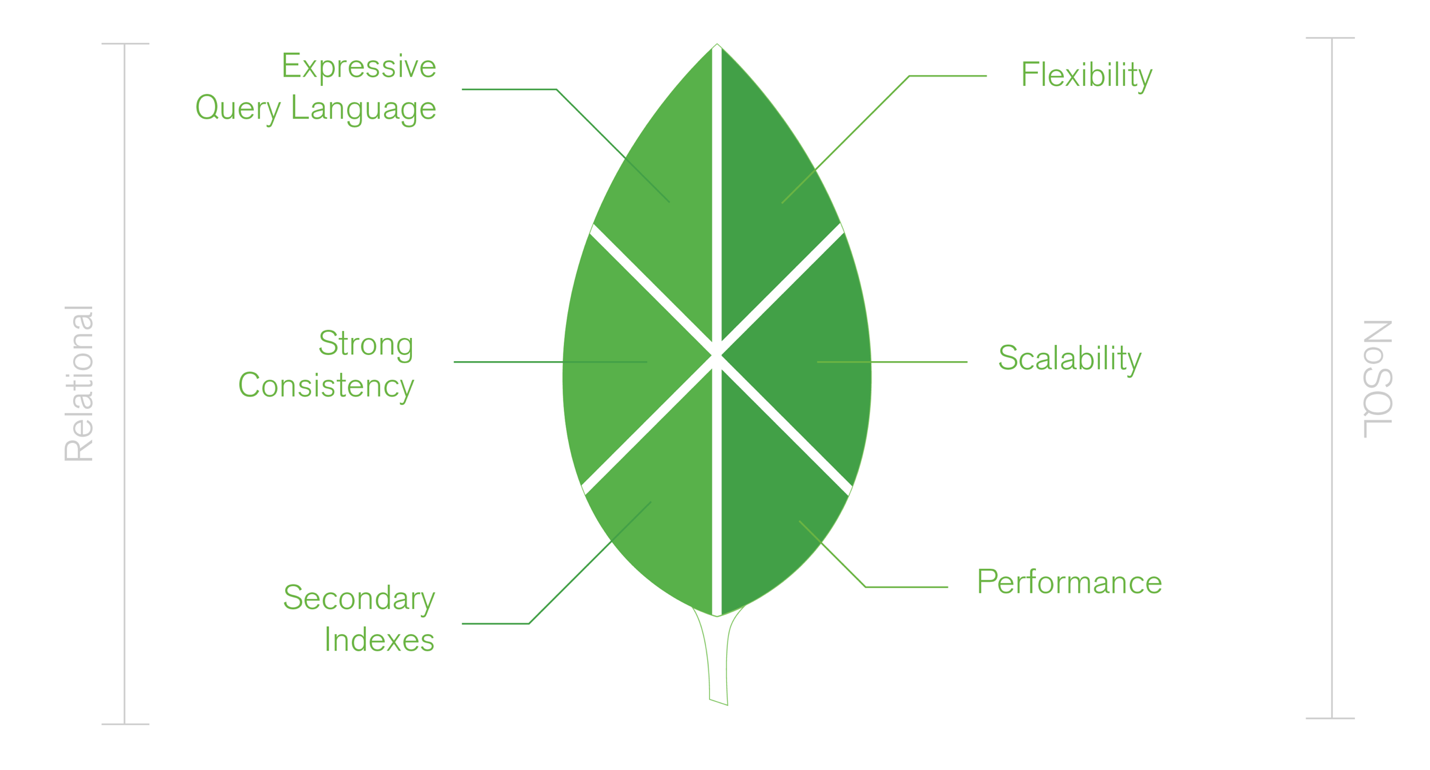
\includegraphics[width=0.9\textwidth]{resources/architectureNoSQLVSRelational}
\caption[MongoDB Architektur]{MongoDB Architektur\protect\footnotemark}
\label{img:architektur}
\end{figure}
\footnotetext{MongoDB Architektur: \url{http://www.moretechnology.de/mongodb-eine-dokumentenorientierte-datenbank/}, zugegriffen am 23. Dezember 2016}

\subsection{CRUD/IFUR}
\subsubsection{Create/Insert}
\begin{listingsboxShell}[label={lst:insert}]{myshell}{Dokument speichern}
> db.collection.insert(..)
\end{listingsboxShell}
\subsubsection{Read/Find}
\begin{listingsboxShell}[label={lst:find}]{myshell}{Dokument finden}
> db.collection.find(..)
> db.collection.findOne(..)
\end{listingsboxShell}
\subsubsection{Update/Update}
\begin{listingsboxShell}[label={lst:update}]{myshell}{Dokument aktualisieren}
> db.collection.update(..)
\end{listingsboxShell}
\subsubsection{Delete/Remove}
\begin{listingsboxShell}[label={lst:remove}]{myshell}{Dokument löschen}
> db.collection.remove(..)
\end{listingsboxShell}
\subsection{Schema Design}
\subsection{Performance}
Siehe in Deutsch über Indexes: \url{https://books.google.de/books?id=kRUbDAAAQBAJ&pg=PA53&lpg=PA53&dq=index+in+mongodb+was+ist+da&source=bl&ots=80Kgw664kZ&sig=rEhHo3g4JRVAVXwUr_In5xzWB8c&hl=en&sa=X&ved=0ahUKEwiBvd_VsbfQAhVDtBQKHX4_ASAQ6AEINjAC#v=onepage&q=index%20in%20mongodb%20was%20ist%20da&f=false}\newline

\subsection{Aggregation Framework}

\subsection{Sharding}\label{sharding}
MongoDB bietet mit AutoSharding ein Feature, das es ermöglicht, einen Datenbankserver automatisch auf verschiedene physikalische Maschinen aufzuteilen und somit die Datenbank horizontal zu skalieren. Um das Sharding bei MongoDB zu konfigurieren, werden drei Komponenten benötigt...., siehe Sharding \url{https://www.iks-gmbh.com/assets/downloads/Einfuehrung-in-MongoDB-iks.pdf
}

\subsection{ODMs für MongoDB}

ODM ist Object-Document Mapper für nichtrelationale Datenbanken wie MongoDB, Apache Cassandra etc.

\subsubsection{Morphia}
Morphia is the Java Object Document Mapper for MongoDB \url{http://mongodb.github.io/morphia/}

\subsubsection{Doctrine}
The Doctrine MongoDB ODM project is a library that provides a PHP object mapping functionality for MongoDB. \url{https://github.com/doctrine/mongodb-odm}

\subsection{Beziehungen}
Folgenden Relationen wie One-to-One \textbf{Teilabschnitt \ref{1:1}}, One-to-Many \textbf{Teilabschnitt \ref{1:n}} und Many-to-Many \textbf{Teilabschnitt \ref{n:m}} blabla

\subsubsection{One-to-One}\label{1:1}
bla

\subsubsection{One-to-Many}\label{1:n}
bla

\subsubsection{Many-to-Many}\label{n:m}
bla

\subsection{Storage Engines}

\subsubsection{MMAPv1}
MMAPv1 is default a storage engine.
MMAPv1 automatically allocates power-of-two-sized documents when new documents are inserted
This is handled by the storage engine.
MMAPv1 is built on top of the mmap system call that maps files into memory
This is the basic idea behind why we call it MMAPv1.

\subsubsection{WiredTiger}

\begin{listingsboxShell}[label={lst:X}]{myshell}{Alle mongod-Prozesse zwingend stoppen}
> killall mongod
\end{listingsboxShell}

Für den Wahl des Storage-Engines \textbf{Wired Tiger} muss man im Terminal den Befehl aus Listing \ref{lst:wiredTiger} ausführen.

\begin{listingsboxShell}[label={lst:wiredTiger}]{myshell}{Something else}
> mongod -dbpath WT --storageEngine wiredTiger
\end{listingsboxShell}

Dann mongo starten mit 'mongo', dann:

\begin{listingsboxShell}[label={lst:X}]{myshell}{Something else}
> db.foo.insert({'name':'andrew'})
\end{listingsboxShell}

\begin{listingsboxShell}[label={lst:X}]{myshell}{Something else}
> db.foo.stats()
\end{listingsboxShell}

\subsection{Indizes}
Indizes in MongoDB werden als Binär-Baum\footnote{Binär-Baum: \url{http://www.hs-augsburg.de/mebib/emiel/entw_inf/lernprogramme/baeume/gdi_kap_4_1.html}, zugegriffen am 23. Dezember 2016} in einer vordefinierten Sortierreihenfolge abgelegt, siehe Abbildung \ref{img:IndexesInMongoDBAreB-Trees}

Der Index wird beim Erstellen, Updaten und Löschen eines Dokumentes auch aktualisiert. Zu viele Indizes machen schreib Operationen langsam und die Größe der Indizes steigt an, deswegen sollte ein Index nur auf Felder zeigen, auf die auch Query-Operationen angewendet werden. Beim Anlegen der Indizes ist die Sortierreihenfolge zu gunsten einer schnelleren Suche wichtig, da sie schon vorsortiert vorliegen und nicht erst bei der Liveabfrage sortiert werden müssen.\footnote{Indizes: \url{http://wikis.gm.fh-koeln.de/wiki_db/MongoDB/Indizes}, aufgerufen am 24. Dezember 2016}

Es gibt drei Möglichkeiten der Sortierung:

\begin{itemize}
\item Aufsteigend(1),
\item Absteigend (-1),
\item geospatial (2d).
\end{itemize}

Index hilft, Datenbanken zu optimieren. Die nachfolgende \autoref{img:EfficiencyofIndexUse} demonstriert

\begin{figure}
\centering
	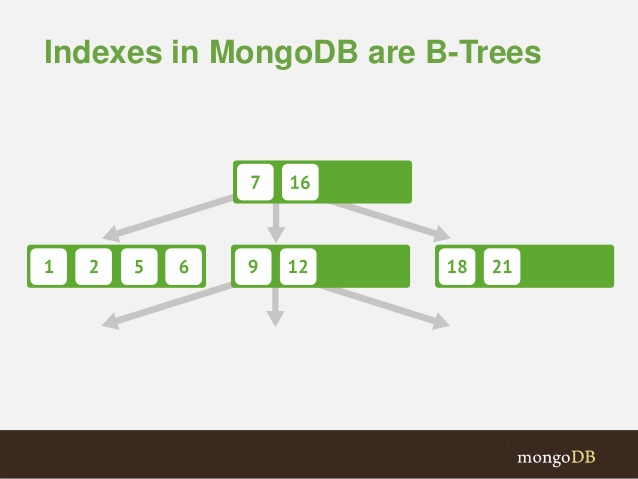
\includegraphics[width=0.7\textwidth]{resources/indexingBtree}
\caption[Indizes in MongoDB als Binär-Baum]{Indizes in MongoDB als Binär-Baum\protect\footnotemark}
\label{img:IndexesInMongoDBAreB-Trees}
\end{figure}
\footnotetext{Indizes in MongoDB als Binä
r-Baum: \url{http://www.slideshare.net/mongodb/indexing-strategies-to-help-you-scale}, zugegriffen am 23. Dezember 2016}

blabla

\begin{figure}
\centering
	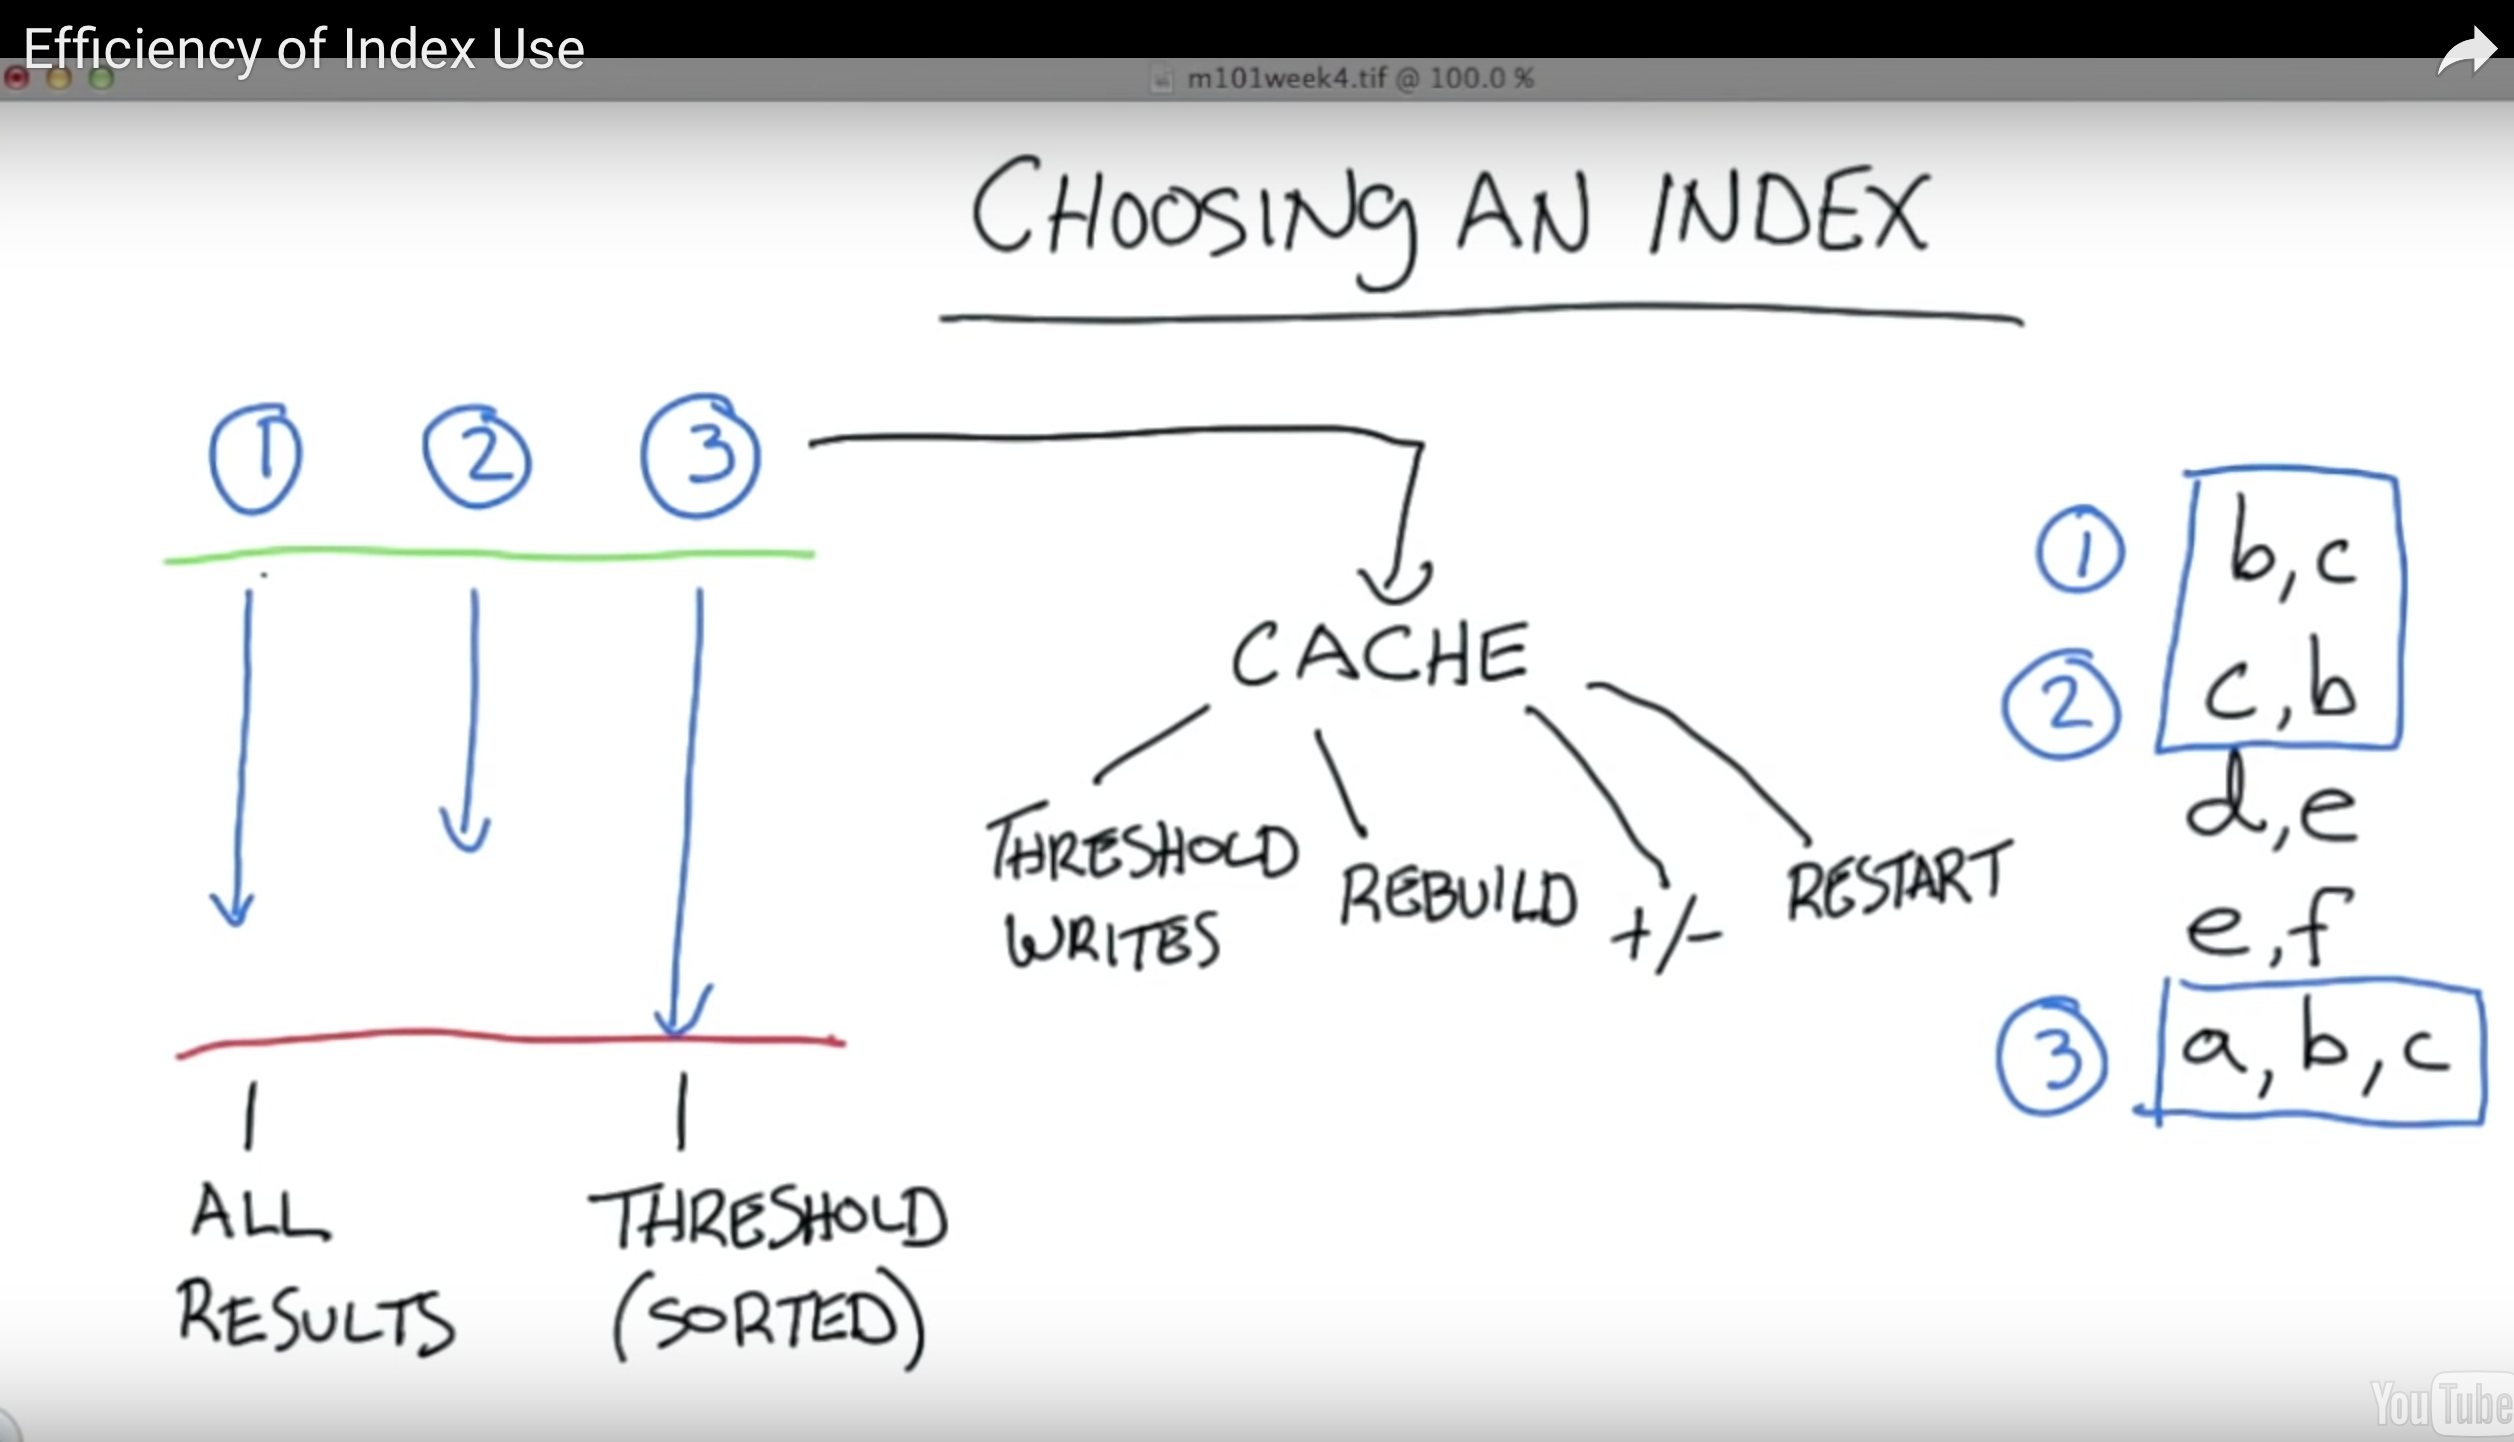
\includegraphics[width=0.7\textwidth]{resources/efficiencyOfIndexUse}
\caption[Efficiency of Index Use]{Efficiency of Index Use\protect\footnotemark}
\label{img:EfficiencyofIndexUse}
\end{figure}
\footnotetext{Efficiency of Index Use: \url{https://docs.mongodb.com/manual/indexes/}, zugegriffen am 12. Dezember 2016}


Neben dem obligatorischen Primär-Index auf dem Feld \_id, das in jedem Dokument existieren und pro Collection eindeutig sein muss, können Sie in MongoDB bis zu 63 weitere Sekundär-Indizes pro Collection anlegen, um Suchanfragen zu beschleunigen. Ein Sekundär-Index kann auf einem einzelnen Feld oder einer Gruppe von Feldern angelegt werden.%\footnote{Indizes: \url{https://www.informatik-aktuell.de/betrieb/datenbanken/mongodb-fuer-software-entwickler.html}}

Which optimization will typically have the greatest impact on the performance of a database?\newline
Adding appropriate indexes on large collections so that only a small percentage of queries need to scan the collection.

\subsection{Creating Indexes}
blabla

\begin{listingsboxShell}[label={lst:X}]{myshell}{Mongo-Shell: Something else}
> db.students.createIndex();
\end{listingsboxShell}

blabla

\begin{listingsboxShell}[label={lst:X}]{myshell}{Mongo-Shell: Something else}
> db.students.explain().find();
\end{listingsboxShell}

Quiz: Please provide the mongo shell command to add an index to a collection named students, having the index key be class, student\_name.
Neither will go in the "-1" direction..

\begin{listingsboxShell}[label={lst:X}]{myshell}{Something else}
> db.students.createIndex({student\_name:1, class:1});
\end{listingsboxShell}

\begin{listingsboxShell}[label={lst:X}]{myshell}{Mongo-Shell: Something else}
> db.students.dropIndex({student_name:1});
\end{listingsboxShell}

\subsubsection{Multikey Indexes}
blabla
\subsubsection{Index Creation Option, Unique}
für jedes attribut kann man Unique definieren, d.h. doppelte Werte dürfen nicht vorkommen\newline\newline

\begin{listingsboxShell}[label={lst:X}]{myshell}{Mongo-Shell: Something else}
> db.students.createIndex({student_id : test}, {unique:true});
\end{listingsboxShell}

Please provide the mongo shell command to create a unique index on student\_id, class\_id, ascending for the collection students.

\begin{listingsboxShell}[label={lst:X}]{myshell}{Mongo-Shell: Something else}
> db.students.createIndex({student_id:1, class_id:1}, {unique:true});
\end{listingsboxShell}

\subsubsection{Index Creation, Sparse}

Im Fall, wenn ein Attribut nicht in allen Dokumenten vorkommt, aber für dieses ein Unique Index definiert werden soll, muss Folgendes verwendet werden:

\begin{listingsboxShell}[label={lst:X}]{myshell}{Something else}
> db.students.createIndex({cell:1}, {unique:true, sparse:true});
\end{listingsboxShell}

blabla, siehe den Shellbefehl, blabla

\begin{listingsboxShell}[label={lst:X}]{myshell}{Something else}
> db.students.createIndex({student_id:1, class_id:1}, {unique:true});
\end{listingsboxShell}
siehe Codeauszug 

\section{Prototyp}
Kommentare zu den Fotos hinzufügen, Eingebettete Kommentare, siehe \url{http://ezproxy.bib.fh-muenchen.de:2125/doi/pdf/10.3139/9783446431225.014}

\section{Aggregation Framework}
How good is it? Mapping between SQL and Aggregation
Um die Nutzung der Aggregation Framework in MongoDB zu ermöglichen, stellt MongoDB Java Driver zur Verfügung. 

\section{Replikation und Verfügbarkeit}
MongoDB kann Server in Replikationsgruppen anordnen, damit bei Ausfall eines Servers die Verfügbarkeit der Datenbank trotzdem gewährleistet ist. In diesem Kapitel werden die Konfigurationsmöglichkeiten für Replikation und Verfügbarkeit der Daten veranschaulicht und zwar wie man Replikation und Verfügbarkeit in MongoDB konfiguriert.
\subsection{Replikation (=Replication)}
blabla

\begin{figure}
\centering
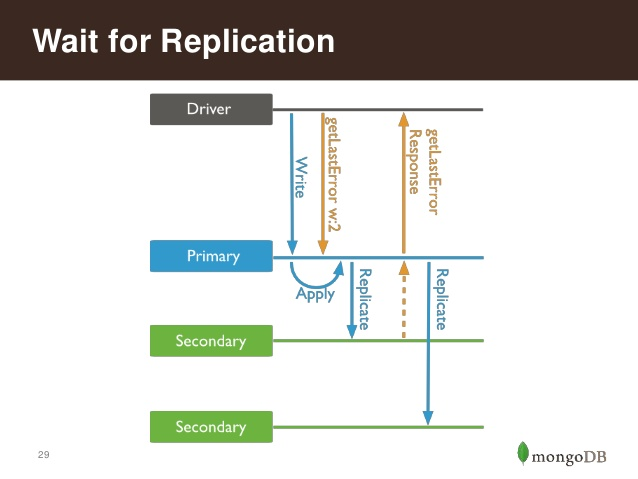
\includegraphics[width=0.7\textwidth]{resources/replication}
\caption[Replikation]{Replikation\protect\footnotemark}
\label{img:Replikation}
\end{figure}
\footnotetext{Replikation: \url{http://www.slideshare.net/mongodb/webinarserie-einfhrung-in-mongodb-back-to-basics-teil-3-interaktion-mit-der-datenbank}, zugegriffen am 18. Dezember 2016}

blabla
\begin{figure}
\centering
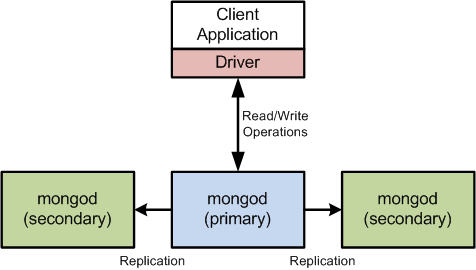
\includegraphics[width=0.7\textwidth]{resources/mongo_replication}
\caption[Master-slave replication in MongoDB]{Master-slave replication in MongoDB\protect\footnotemark}
\label{img:mongo_replication}
\end{figure}
\footnotetext{Master-slave replication in MongoDB: \url{http://spichale.blogspot.de/2013/08/replication-in-mongodb-concepts-and.html}, zugegriffen am 29. Dezember 2016}



Typen von Replikationsgruppen:
\begin{itemize}
\item Regular
\item Arbiter
\item Delayed/Regular
\item Hidden
\end{itemize}
\subsection{Erstellen von Replikationsgruppen}

\begin{listingsboxShell}[label={lst:scriptForCreateOfRep}]{myshell}{Skript fürs Erstellen einer Replikationsgruppe}
#!/usr/bin/env bash

mkdir -p /data/rs1 /data/rs2 /data/rs3

// Start von drei lokalen mongod-Instanzen als Replikationsgruppe

mongod --replSet m101 --logpath "1.log" --dbpath /data/rs1 --port 27017
--oplogSize 64 --fork --smallfiles
mongod --replSet m101 --logpath "2.log" --dbpath /data/rs2 --port 27018
--oplogSize 64 --smallfiles --fork
mongod --replSet m101 --logpath "3.log" --dbpath /data/rs3 --port 27019
--oplogSize 64 --smallfiles --fork
\end{listingsboxShell}

Das Skript mit dem Inhalt aus Listing \ref{lst:scriptForCreateOfRep} ist mit dem aus Listing \ref{lst:runOfscriptForCreateOfRep} auszuführen:

\begin{listingsboxShell}[label={lst:runOfscriptForCreateOfRep}]{myshell}{Erstellen einer Replikationsgruppe anhand eines Skriptes}
vlfa:scripts vlfa$ bash < create_replica_set.sh
\end{listingsboxShell}

Bei der Ausführung des Skriptes kann zu den Problemen führen. Um aktuelle Prozesse mit mongo anschauen und stoppen zu können, muss man folgenden Befehl angeben. The problem was that I have runned mongod without any parameters before I started launching the nodes. First kill all the mongo, mongod and mongos instances to guarantee the environment is clear.\url{http://stackoverflow.com/questions/25839559/mongodb-server-is-not-running-with-replset}

\begin{listingsboxShell}[label={lst:listOfPIDs}]{myshell}{Auflistung aktueller mongo(s,d)-Prozesse}
vlfa:scripts vlfa$ ps -ef | grep 'mongo'
\end{listingsboxShell}

Danach ist wichtig, Prozesse zu stoppen. Dafür muss man nach dem Befehl kill die ProzessID eingeben, siehe Listing \ref{lst:killPID}. Dann wird die Möglichkeit fürs Erstellen eigener Replikationsgruppe ermöglicht, siehe dazu Listings \ref{lst:scriptForCreateOfRep} und \ref{lst:runOfscriptForCreateOfRep}.

\begin{listingsboxShell}[label={lst:killPID}]{myshell}{mongo(s,d)-Server zwingend stoppen}
// konkreten mongo(s,d)-Server zwingend stoppen
vlfa:scripts vlfa$ kill 'PID'

// alle mongo(s,d)-Server zwingend stoppen
vlfa:scripts vlfa$ killall mongo(s,d)
\end{listingsboxShell}

Damit ist die Konfigurationsgruppe mit 3 Servern angelegt. Zum Anschauen einer log-Datei;

\begin{listingsboxShell}[label={lst:X}]{myshell}{1.log-Inhalt}
2016-12-19T14:58:11.637+0100 I CONTROL  [initandlisten] MongoDB starting :
pid=25626 port=27017 dbpath=/data/rs1 64-bit host=vlfa.fritz.box
// irrelevant
2016-12-19T14:58:11.639+0100 I CONTROL  [initandlisten] options:
{ net: { port: 27017 }, processManagement: { fork: true }, replication:
{ oplogSizeMB: 64, replSet: "m101" }, storage: { dbPath: "/data/rs1",
mmapv1: {smallFiles: true}}, systemLog: {destination: "file", path: "1.log"}}
// irrelevant
\end{listingsboxShell}
Die Replikationsgruppe starten.......blabla
\begin{listingsboxJavaScript}[label={lst:initReplica}]{myJS}{Skript zum Start der Replikationsgruppe}
config = { _id: "m101", members:[
          { _id : 0, host : "localhost:27017", priority:0, slaveDelay:5},
          { _id : 1, host : "localhost:27018"},
          { _id : 2, host : "localhost:27019"} ]
};

rs.initiate(config);
rs.status();
\end{listingsboxJavaScript}

Die Server aus Listing \ref{lst:initReplica} nehmen nun Kontakt miteinander auf, gründen die Gruppe und wählen den Primary-Server aus. Wie im Skript aus Listing 	\ref{lst:initReplica} zu entnehmen ist, kann der Zustand der Replikationsgruppe mit \texttt{rs.status()} geprüft werden. Bei Ausfall des Primary-Servers wählen die Secondaries untereinander entsprechend einen neuen Primary-Server. Damit wird die Ausfallsicherheit des Servers erreicht. Die Mindestanzahl an Server in einer Replikationsgruppe liegt bei drei. 

\begin{listingsboxShell}[label={lst:runOfInitReplica}]{myshell}{Skript ausführen}
vlfa:scripts vlfa$ mongo --port 27018 < init_replica.js
\end{listingsboxShell}

Die Priorität '0' teilt mit, wer Primary Member in der Replikationsgruppe ist. Korrigieren, Stimmt nicht....\url{https://docs.mongodb.com/v3.2/core/replica-set-priority-0-member/}

\begin{listingsboxJava}[label={lst:X}]{myJava}{Skript zur Initialisierung der Replikationsgruppe}
public static void main (String[] args) throws InterruptedException {
        MongoClient client = new MongoClient(asList(
                new ServerAddress("localhost", 27017),
                new ServerAddress("localhost", 27018),
                new ServerAddress("localhost", 27019)));
                
                // weitere Operationen
}
\end{listingsboxJava}

\begin{listingsboxShell}[label={lst:X}]{myshell}{Simulation des Server-Ausfalls 'PRIMARY'}
m101:PRIMARY> rs.stepDown()

Result:

2016-12-19T21:24:12.739+0100 I NETWORK  [thread1]
trying reconnect to 127.0.0.1:27018 (127.0.0.1) failed
2016-12-19T21:24:12.760+0100 I NETWORK  [thread1]
reconnect 127.0.0.1:27018 (127.0.0.1) ok
m101:SECONDARY> 
\end{listingsboxShell}

Der aktuelle MongoDB Java Treiber ist in Version 3.4.0 verfügbar und kann bequem als Maven Dependency geladen werden, siehe Listing  \ref{lst:mongoJDriver}.
 
\begin{listingsboxJava}[label={lst:mongoJDriver}]{myxml}{MongoDB Java Treiber in Version 3.4.0 als Maven Dependency}
<dependency>
        <groupId>org.mongodb</groupId>
        <artifactId>mongo-java-driver</artifactId>
        <version>3.4.0</version>
</dependency>
\end{listingsboxJava}




Um die Sicherung der Zugehörigkeit der Mitglieder zu konkreter Replikationsgruppe festzustellen, siehe Listing \ref{lst:guarantee}, Zeilen 6-8...
\begin{listingsboxJava}[label={lst:guarantee}]{myJava}{Sicherung der Zugehörigkeit zu konkreter Replikationsgruppe}
 public static void main (String[] args) throws InterruptedException {
        MongoClient client = new MongoClient(asList(
                new ServerAddress("localhost", 27017),
                new ServerAddress("localhost", 27018),
                new ServerAddress("localhost", 27019)), 
                MongoClientOptions.builder()
                        .requiredReplicaSetName("m101")
                        .build());
\end{listingsboxJava}



\section{Fazit}
Siehe Listing \ref{lst:X} \newline 
Doch wie der Begriff Not only SQL (NoSQL) andeutet, stehen beide Datenbanksysteme nicht unbedingt in direkter Konkurrenz zueinander, sondern können sich gegenseitig ergänzen. Dennoch, wenn es um die persistente Datenspeicherung bei Web-Anwendungen geht, stellen relationale Datenbanken nicht mehr die einzige Alternative dar. Bei eigenen Projekten wären Entwickler heute also gut beraten, die Vor- und Nachteile der beiden Systeme gegenüberzustellen und entsprechend den eigenen Anforderungen und Prioritäten zu bewerten. Muss das System mit großen Datenmengen effizient umgehen können? Werden hohe Anforderungen an Skalierbarkeit und Flexibilität der Datenbank gestellt? Sollen sich die Daten über mehrere Server verteilen lassen? Sind häufige Änderungen an der Datenstruktur in Zukunft zu erwarten? Wenn Sie die meisten dieser Fragen mit "Ja" beantworten, dann sollten Sie sich MongoDB zumindest näher anschauen.\newline\newline

Daten in MongoDB verfügen über ein flexibles Schema. Kollektionen (=Collections) erzwingt keine Struktur.

\begin{listingsboxJava}[label={lst:conn}]{myJava}{Verbindungsaufbau}
public static void main(String[] args) {

	MongoClient mongoClient = new MongoClient("localhost", 27017);
        MongoDatabase db = mongoClient.getDatabase("test");
        MongoCollection<Document> collectionOfZips = db.getCollection("zips");
        
        // weitere CRUD-Operationen mit der ausgewählten Kollektion
}
\end{listingsboxJava}
\subsection{Sharding und Verfügbarkeit}
Die Datenmengen in Form von Blöcken (=Chunks) wird auf \texttt{n-}Knoten verteilt. Jedes Dokument landet auf genau einem Knoten. Auf jedes Dokument wird über sog. ShardKey zugegriffen. ShardKey muss bei der Erstellung des Sharding-Systems angegeben werden. Bei der Angabe des Shard-Keys muss Folgendes ...???? berücksichtigt werden. Das Ziel des Ganzen ist die horizontale Skalierbarkeit an Datenmengen.



Test \ref{lst:conn}
\section{Apache Cassandra}
Cassandra\footnote{Apache Cassandra: \url{http://cassandra.apache.org}, zugegriffen am 16. Dezember 2016} zählt, neben MongoDB\footnote{MongoDB: \url{https://www.mongodb.com}, zugegriffen am 16. Dezember 2016}, zu den derzeit populärsten NoSQL-Datenbanken. Cassandra war ursprünglich eine proprietäre Datenbank von Facebook und wurde 2008 als Open-Source-Datenbank veröffentlicht. Beispiele für weitere NoSQL-Datenbanken sind SimpleDB\footnote{SimpleDB: \url{https://aws.amazon.com/de/simpledb/}, zugegriffen am 16. Dezember 2016}, Google Big Table\footnote{Google Big Table: \url{https://research.google.com/archive/bigtable.html}, zugegriffen am 16. Dezember 2016}, Apache Hadoop\footnote{Apache Hadoop: \url{http://hadoop.apache.org}, zugegriffen am 16. Dezember 2016}, MapReduce\footnote{MapReduce: \url{http://hortonworks.com/apache/mapreduce/}, zugegriffen am 16. Dezember 2016}, MemcacheDB\footnote{MemcacheDB: \url{http://memcachedb.org}, zugegriffen am 16. Dezember 2016} und Voldemort\footnote{Voldemort: \url{http://www.project-voldemort.com/voldemort/}, zugegriffen am 16. Dezember 2016}. Unternehmen, die auf NoSQL setzen, sind unter anderem NetFlix\footnote{NetFlix: \url{https://www.netflix.com/de-en/}}, LinkedIn\footnote{LinkedIn: \url{https://www.linkedin.com/feed/}} und Twitter\footnote{Twitter: \url{https://twitter.com/?lang=en}}.\footnote{NoSQL: \url{http://www.searchenterprisesoftware.de/definition/NoSQL}, zugegriffen am 16. Dezember 2016}\newline

Cassandra ist als skalierbares, ausfallsicheres System für den Umgang mit großen Datenmengen auf verteilten Systemen (Clustern) konzipiert. Sie ist die beliebteste spaltenorientierte NoSQL-Datenbank und im Gegensatz zu MongoDB (C++) in Java geschrieben. Aufgrund ihrer architektonischen Eigenschaften wird Cassandra häufig in Big-Data-Projekten eingesetzt, kann in Zusammenarbeit mit einem Applikations-Server/Framework aber auch gut für komplexe Webanwendungen verwendet werden.
 \clearpage
\chapter{Prototyp}

\begin{listingsboxShell}[label={lst:X}]{myshell}{Alle mongod-Prozesse zwingend stoppen}
> killall mongod
\end{listingsboxShell}


\section{Prototyp}
Kommentare zu den Fotos hinzufügen, Eingebettete Kommentare, siehe \url{http://ezproxy.bib.fh-muenchen.de:2125/doi/pdf/10.3139/9783446431225.014}



\section{Fazit}
Siehe Listing \ref{lst:X} \newline 
Doch wie der Begriff Not only SQL (NoSQL) andeutet, stehen beide Datenbanksysteme nicht unbedingt in direkter Konkurrenz zueinander, sondern können sich gegenseitig ergänzen. Dennoch, wenn es um die persistente Datenspeicherung bei Web-Anwendungen geht, stellen relationale Datenbanken nicht mehr die einzige Alternative dar. Bei eigenen Projekten wären Entwickler heute also gut beraten, die Vor- und Nachteile der beiden Systeme gegenüberzustellen und entsprechend den eigenen Anforderungen und Prioritäten zu bewerten. Muss das System mit großen Datenmengen effizient umgehen können? Werden hohe Anforderungen an Skalierbarkeit und Flexibilität der Datenbank gestellt? Sollen sich die Daten über mehrere Server verteilen lassen? Sind häufige Änderungen an der Datenstruktur in Zukunft zu erwarten? Wenn Sie die meisten dieser Fragen mit "Ja" beantworten, dann sollten Sie sich MongoDB zumindest näher anschauen.\newline\newline

Daten in MongoDB verfügen über ein flexibles Schema. Kollektionen (=Collections) erzwingt keine Struktur.



\section{Apache Cassandra}
Cassandra\footnote{Apache Cassandra: \url{http://cassandra.apache.org}, zugegriffen am 16. Dezember 2016} zählt, neben MongoDB\footnote{MongoDB: \url{https://www.mongodb.com}, zugegriffen am 16. Dezember 2016}, zu den derzeit populärsten NoSQL-Datenbanken. Cassandra war ursprünglich eine proprietäre Datenbank von Facebook und wurde 2008 als Open-Source-Datenbank veröffentlicht. Beispiele für weitere NoSQL-Datenbanken sind SimpleDB\footnote{SimpleDB: \url{https://aws.amazon.com/de/simpledb/}, zugegriffen am 16. Dezember 2016}, Google Big Table\footnote{Google Big Table: \url{https://research.google.com/archive/bigtable.html}, zugegriffen am 16. Dezember 2016}, Apache Hadoop\footnote{Apache Hadoop: \url{http://hadoop.apache.org}, zugegriffen am 16. Dezember 2016}, MapReduce\footnote{MapReduce: \url{http://hortonworks.com/apache/mapreduce/}, zugegriffen am 16. Dezember 2016}, MemcacheDB\footnote{MemcacheDB: \url{http://memcachedb.org}, zugegriffen am 16. Dezember 2016} und Voldemort\footnote{Voldemort: \url{http://www.project-voldemort.com/voldemort/}, zugegriffen am 16. Dezember 2016}. Unternehmen, die auf NoSQL setzen, sind unter anderem NetFlix\footnote{NetFlix: \url{https://www.netflix.com/de-en/}}, LinkedIn\footnote{LinkedIn: \url{https://www.linkedin.com/feed/}} und Twitter\footnote{Twitter: \url{https://twitter.com/?lang=en}}.\footnote{NoSQL: \url{http://www.searchenterprisesoftware.de/definition/NoSQL}, zugegriffen am 16. Dezember 2016}\newline

Cassandra ist als skalierbares, ausfallsicheres System für den Umgang mit großen Datenmengen auf verteilten Systemen (Clustern) konzipiert. Sie ist die beliebteste spaltenorientierte NoSQL-Datenbank und im Gegensatz zu MongoDB (C++) in Java geschrieben. Aufgrund ihrer architektonischen Eigenschaften wird Cassandra häufig in Big-Data-Projekten eingesetzt, kann in Zusammenarbeit mit einem Applikations-Server/Framework aber auch gut für komplexe Webanwendungen verwendet werden.
 \clearpage
%\chapter{Fachkonzeptschicht}
blabla
\colorbox{red}{BILD nur zum Testennnnnnn}
\begin{figure}
\centering
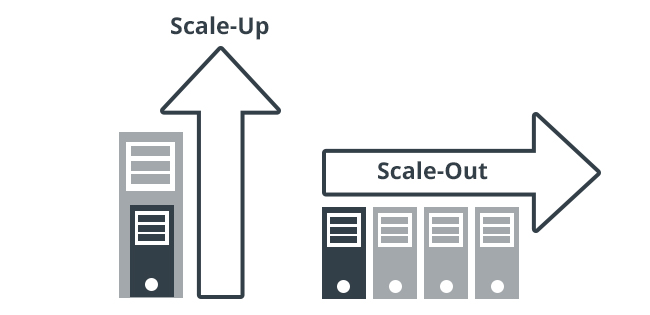
\includegraphics[width=0.7\textwidth]{resources/scales}
\caption[TEST]{TEST\protect\footnotemark}
\label{img:scales}
\end{figure}
\footnotetext{TEST: \url{https://magazin.kapilendo.de/den-supergau-verhindern-so-bereiten-sie-ihre-website-auf-einen-besucheransturm-vor/}, zugegriffen am 15. Januar 2017}
\section{Allgemein}

\begin{listingsboxJava}[label={lst:X}]{myJava}{Skript zur Initialisierung der Replikationsgruppe}
bla
\end{listingsboxJava} \clearpage
%\chapter{GUI-Schicht}
blabla
\section{Allgemein} \clearpage
%\chapter{Eine Cloud-Fotoalben-Verwaltung}
\section{Fachliche Spezifikation für die Endbenutzer}
Die folgende Spezifikation hat das Ziel, dem Endbenutzer die Grundprinzipien der geplanten webbasierten skalierbaren Anwendung für Fotoalben-Verwaltung zu präsentieren.
Die skalierbare Software für die webbasierte Fotoalben-Verwaltung ist geplant so zu implementieren, dass jeder sie als eigene Fotoalben-Verwaltung nutzen kann, unabhängig von wachsenden Ansprüchen an die Leistungsfähigkeit. 

\section{Anwendungsfälle}
Im Folgenden sind alle möglichen Szenarien dargestellt, die bei der Interaktion zwischen dem Besucher/Benutzer und des betrachteten Systems vorkommen können.

\subsection{Vorschau aller öffentlichen Fotoalben}
\begin{usecase}
\addtitle{Vorschau aller öffentlichen Fotoalben (=Preview of all public photo albums)}{}

\addfield{Kurzbeschreibung:}{Jeder Besucher kann alle vorhandenen öffentlichen Fotoalben sehen}
\addfield{Auslöser:}{Der Besucher verwendet den ihm bekannten Link für die Cloud-Fotoalben-Verwaltung}
\addfield{Eingabe:}{Den funktionierenden Link für die Cloud-Fotoalben-Verwaltung im Browser}
\addfield{Vorbedingung:}{Das System ist deployed}
\addfield{Ergebnis:}{Der Besucher landet auf die webbasierte Cloud-Fotoalben-Verwaltung und kann alle vorhandenen öffentlichen Fotoalben sehen}

\end{usecase}

\subsection{Fotoalbum ansehen}
\begin{usecase}
\addtitle{Ein Fotoalbum auswählen (= Show a photo album)}{}

\addfield{Kurzbeschreibung:}{Jeder Besucher kann den Inhalt jedes öffentlichen Fotoalbums ansehen}
\addfield{Auslöser:}{Der Besucher klickt auf das entsprechende Fotoalbum an, um seinen Inhalt ansehen zu können}
\addfield{Eingabe:}{\textbf{keine}}
\addfield{Vorbedingung:}{mind. ein Fotoalbum existiert}
\addfield{Ergebnis:}{Der Besucher kann den Inhalt des Fotoalbums sehen}

\end{usecase}

\subsection{Foto im Vollformat ansehen}
\begin{usecase}
\addtitle{Ein Foto im Vollformat ansehen (Show a photo in the full format)}{}

\addfield{Kurzbeschreibung:}{Jeder Besucher kann jedes Foto im Vollformat sehen}
\addfield{Auslöser:}{Der Besucher klickt auf das entsprechende Foto an, um es im Vollformat ansehen zu können}
\addfield{Eingabe:}{\textbf{keine}}
\addfield{Vorbedingung:}{mind. ein Foto existiert}
\addfield{Ergebnis:}{Der Besucher kann im Vollformat das Foto ansehen}

\end{usecase}

\subsection{Benutzerregistrierung}
\begin{usecase}
\addtitle{Registrierung (=Register)}{}

\addfield{Kurzbeschreibung:}{Ein Besucher registriert sich als neuer Benutzer }
\addfield{Auslöser:}{Der potentielle Benutzer klickt auf den Button \textbf{'Register'} und legt ein neues Benutzerkonto selbst an}
\addfield{Eingabe:}{Benutzername, Passwort und E-Mail sind für die Registrierung unbedingt einzugeben}
\addfield{Vorbedingung:}{Der potentielle Benutzer ist unter dem eingegebenen Benutzername im System noch nicht registriert}
\addfield{Ergebnis:}{Das Benutzerkonto für den neuen Benutzer wird im System angelegt. Der Benutzer wird nach der \textbf{'Registrierung'} an die Startseite weitergeleitet}

\end{usecase}

\subsection{Benutzeranmeldung}
\begin{usecase}
\addtitle{Anmeldung (=Login)}{}

\addfield{Kurzbeschreibung:}{Der registrierte Benutzer meldet sich im System an}
\addfield{Auslöser:}{Für die Anmeldung klickt der Benutzer auf den Button \textbf{'Please login'} und meldet sich mit seinem Benutzername und Passwort im System an}
\addfield{Eingabe:}{Benutzername und Passwort}
\addfield{Vorbedingung:}{Der Benutzer ist im System schon registriert}
\addfield{Ergebnis:}{Der Benutzer wird nach der erfolgreichen Anmeldung an eigene Startseite weitergeleitet}

\end{usecase}

\subsection{Fotoalbum anlegen}
\begin{usecase}
\addtitle{Fotoalbum anlegen (=Create a new photo album)}{}

\addfield{Kurzbeschreibung:}{Der angemeldete Benutzer legt sein neues Fotoalbum an}
\addfield{Auslöser:}{Für die Erzeugung eines neuen Fotoalbums klickt der Benutzer auf den Button \textbf{'Create a new photo album'}}
\addfield{Eingabe:}{Bezeichnung, Beschreibung und Abgrenzungsoption (= privat oder öffentlich) für sein zukünftiges Fotoalbum}
\addfield{Vorbedingung:}{Das Fotoalbum mit so einem Namen existiert bei dem angemeldeten Benutzer \textbf{nicht}}
\addfield{Ergebnis:}{Das Fotoalbum wird erzeugt und die Möglichkeit für das \textbf{'Select a photo for upload'} wird gleich freigeschaltet}

\end{usecase}

\subsection{Foto hochladen}
\begin{usecase}
\addtitle{Foto hochladen (=Upload a photo)}{}

\addfield{Kurzbeschreibung:}{Ein Benutzer lädt Fotos in ein existierendes Fotoalbum hoch}
\addfield{Auslöser:}{Für das Hochladen von Fotos in ein Fotoalbum klickt der Benutzer auf den Button \textbf{'Select a photo for upload'} und wählt ein Foto zum Hochladen aus}
\addfield{Eingabe:}{Gewünschtes Foto zum Hochladen auswählen}
\addfield{Vorbedingung:}{mind. ein Fotoalbum existiert}
\addfield{Ergebnis:}{Das ausgewählte Foto wird hochgeladen und die Möglichkeit für das \textbf{'Play a slideshow'} wird mit dem 1. hochgeladenen Foto gleich freigeschaltet}

\end{usecase}

\subsection{Foto löschen}
\begin{usecase}
\addtitle{Foto löschen (=Delete a photo)}{}

\addfield{Kurzbeschreibung:}{Nur ein registrierter Benutzer kann die eigenen Fotos aus den Fotoalben löschen}
\addfield{Auslöser:}{Für das Löschen von Fotos in einem Fotoalbum wählt der Benutzer bestimmte Fotos aus einem Fotoalbum aus und klickt auf den Button \textbf{'Delete n photos'}. \textbf{n} steht für die Anzahl von Fotos}
\addfield{Eingabe:}{\textbf{keine}}
\addfield{Vorbedingung:}{Die löschenden Fotos existieren}
\addfield{Ergebnis:}{Die markierten Fotos sind gelöscht und sind in dem Fotoalbum nicht mehr vorhanden}

\end{usecase}

\subsection{Fotoalbum löschen}
\begin{usecase}
\addtitle{Fotoalbum löschen (=Delete a photo album)}{}

\addfield{Kurzbeschreibung:}{Nur ein registrierter Benutzer kann die eigenen oder für ihn sichtbaren Fotoalben mit dem ganzen Inhalt löschen}
\addfield{Auslöser:}{Für das Löschen von Fotoalben klickt der Benutzer auf den Button \textbf{'Delete a photo album'}}
\addfield{Eingabe:}{\textbf{keine}}
\addfield{Vorbedingung:}{Das löschende Fotoalbum existiert}
\addfield{Ergebnis:}{Das Fotoalbum ist gelöscht und ist im System nicht mehr vorhanden}

\end{usecase}

\subsection{Foto-Diashow abspielen - \textbf{optional}}
\begin{usecase}
\addtitle{Foto-Diashow abspielen (=Play a slideshow)}{}

\addfield{Kurzbeschreibung:}{Ein Benutzer spielt Foto-Diashow ab}
\addfield{Auslöser:}{Für das Abspielen von Foto-Diashow klickt der Benutzer auf den Button \textbf{'Play a slideshow'}}
\addfield{Eingabe:}{\textbf{keine}}
\addfield{Vorbedingung:}{mind. ein Foto ist in einem Fotoalbum vorhanden}
\addfield{Ergebnis:}{Der Benutzer kann Foto-Diashow abspielen}

\end{usecase}

\subsection{Fotoalbum freigeben - \textbf{optional}}
\begin{usecase}
\addtitle{Fotoalbum freigeben (=Share a photo album)}{}

\addfield{Kurzbeschreibung:}{Ein Benutzer lädt seine Bekannte/Freunde/Verwandte zum einem bestimmten Fotoalbum per E-Mail ein, um dieses verwalten zu können}
\addfield{Auslöser:}{Für die Freigabe eines Fotoalbums klickt der Benutzer auf den Button \textbf{'Share a photo album'} und teilt per E-Mail über die Freigabe des Fotoalbums an die Gewünschten mit}
\addfield{Eingabe:}{Die E-Mail-Adressen von Bekannten/Freunden/Verwandten für die Freigabe}
\addfield{Vorbedingung:}{Der Eingeladene befindet sich nicht in der Liste der Freigegebenen}
\addfield{Ergebnis:}{Der Eingeladene kann ein freigegebenes Fotoalbum verwalten}

\end{usecase}

\subsection{Fotoalbum als Gast verwalten - \textbf{optional}}
\begin{usecase}
\addtitle{Fotoalbum als Gast verwalten (=Manage a photo album as guest)}{}

\addfield{Kurzbeschreibung:}{Ein Gast kann die für ihn freigegebenen Fotoalben verwalten}
\addfield{Auslöser:}{Eine Einladung per E-Mail, die eine Freigabe in Form eines Links verfügt}
\addfield{Eingabe:}{\textbf{keine}}
\addfield{Vorbedingung:}{Eine Freigabe per E-Mail}
\addfield{Ergebnis:}{Der eingeladene Gast kann das für ihn freigegebene Fotoalbum verwalten}

\end{usecase}

\subsection{Foto kommentieren - \textbf{optional}}
\begin{usecase}
\addtitle{Foto kommentieren (=Comment on a photo)}{}

\addfield{Kurzbeschreibung:}{Nur ein autorisierter Benutzer kann Fotos kommentieren}
\addfield{Auslöser:}{Für das Kommentieren von Fotos gibt der autorisierter Benutzer auf den Button \textbf{'Comment'} und gibt seinen Kommentar ein}
\addfield{Eingabe:}{Seine Meinung zu dem gewählten Foto}
\addfield{Vorbedingung:}{mind. ein Foto ist in einem Fotoalbum vorhanden und der Benutzer darf nicht unauthentifiziert sein}
\addfield{Ergebnis:}{Das Foto verfügt über einen \textbf{neuen} Kommentar}

\end{usecase}

%\subsection{}
%\begin{usecase}
%\addtitle{}{}
%
%\addfield{Kurzbeschreibung:}{}
%\addfield{Auslöser:}{}
%\addfield{Eingabe:}{}
%\addfield{Vorbedingung:}{}
%\addfield{Ergebnis:}{}
%
%\end{usecase}

%\section{Technische Spezifikation für die Entwickler}

%Eine technische Spezifikation dient dem Entwickler zur Orientierung, wie die geplante Software strukturiert ist und wie die in der Abbildung XXX dargestellten Module zusammenspielen, welche Frameworks, Programmiersprachen für Frontend und Backend genutzt werden.

 \clearpage

\pagenumbering{Alph}
\printbibliography[heading=bibintoc, keyword={book}, title={Literaturverzeichnis}]\clearpage
\printbibliography[heading=bibintoc, keyword={online}, title={Onlinequellen}]\clearpage

\listoffigures \clearpage
%\listoftables \clearpage
\printbibliography[heading=bibintoc, keyword={image}, title={Bildquellen}]\clearpage
\tcblistof[\chapter*]{mybox}{Quelltextverzeichnis}

\end{document}